\setcounter{tocdepth}{1}
\setlist[itemize]{leftmargin=1.4em,itemsep=2pt,topsep=4pt}
\setlist[enumerate]{leftmargin=1.5em,itemsep=2pt,topsep=4pt}
\captionsetup{font=small,labelfont=bf}
\pagestyle{fancy}
\fancyhf{}
\fancyhead[L]{\small CO3133 -- Assignment 1}
\fancyhead[R]{\small Group G-M10}
\fancyfoot[C]{\thepage}
\renewcommand{\headrulewidth}{0.3pt}
\setlength{\headheight}{14pt}

\begin{titlepage}
\centering
{\large VIETNAM NATIONAL UNIVERSITY HO CHI MINH CITY\par}
\vspace{4mm}
{\Large\bfseries HO CHI MINH CITY UNIVERSITY OF TECHNOLOGY\par}
\vspace{3mm}
{\large Faculty of Computer Science and Engineering\par}
\vspace{21mm}
{\large CO3133 -- Deep Learning and Its Applications\par}
\vspace{7mm}
{\Huge\bfseries Fashion-MNIST Classification\par}
\vspace{7mm}
{\LARGE Architectures and Controlled Training Studies\par}
\vspace{4mm}
{\large With an RGB Garment Classification Extension\par}
\vspace{12mm}
{\Large Assignment 1 -- Final Report\par}
\vspace{15mm}
\begin{tabular}{ll}
\textbf{Group} & G-M10 \\
\textbf{Members} & Trần Gia Lâm -- 2352670 \\
 & Nguyễn Hữu Cầu -- 2352129 \\
\textbf{Instructor} & Lê Thành Sách \\
\textbf{Semester} & 261 \\
\end{tabular}
\vfill
{\large Ho Chi Minh City, October 2026\par}
\end{titlepage}

\pagenumbering{roman}
\section*{Abstract}
We compare a linear classifier, multilayer perceptron, custom CNN, row-wise GRU and patch Transformer on Fashion-MNIST using fixed partitions and a shared PyTorch pipeline. The original 20-epoch study selects checkpoints by validation cross-entropy before official-test evaluation. CNN records the highest test accuracy among these five models, 89.59\%. Later optimization remains separate because the official test was already inspected.

A 61-fit recipe search yields CNN validation Macro-F1 $0.93308\pm0.00027$ over three seeds. A subsequent matched study completes 30 fits and retains 90 checkpoints, comparing the original and selected recipes at minimum cross-entropy, maximum F1 and fixed epoch 60. The predeclared primary CNN contrast at epoch 60 is $+0.000912$ mean F1, with a paired SD of $0.003511$ and a positive difference in one of three seeds. This result does not establish a reliable CNN recipe gain. MLP and Transformer show more consistent positive differences at the fixed horizon. All follow-up Fashion-MNIST scores use previously inspected validation images.

An optional six-class Fashionpedia extension uses ImageNet-initialized MobileNetV3-Small, grouped data roles and calibrated selective prediction. Fine-tuning outperforms a frozen encoder on the original assessment, but a later dropout study does not establish a further gain there. A prospectively locked source-cohort audit evaluates six fixed models on 2,766 project-unused crops in 1,826 source/duplicate components. Mean F1 is 0.77449 for C0 and 0.78154 for C4, with paired difference $0.00705$ and a component-bootstrap interval $[-0.00036,0.01512]$. The interval includes zero. The preset C4 policy accepts 54.45\% of crops with 95.95\% observed accepted accuracy, without retuning. A post-hoc class analysis finds accepted accuracy of 66.67\% for true shirt/blouse crops and accepted precision of 86.36\% for outputs labeled jacket, exposing weaknesses hidden by the pooled rate. This license-defined population shift does not certify arbitrary future images.

Saved predictions, configurations and checkpoints support independent numerical checks. Local PyTorch serving passes its recorded regression and HTTP checks, while broader ONNX parity remains unresolved. The experiments distinguish recipe effects, checkpoint selection and population changes, retaining negative results and explicit limits on generalization and numerical portability.

\clearpage
\begingroup\small\setlength{\parskip}{0pt}
\makeatletter\renewcommand{\l@section}{\@dottedtocline{1}{0em}{2.2em}}\makeatother
\tableofcontents
\endgroup
\clearpage
\pagenumbering{arabic}
\part{Problem, data and evaluation}
\section{Problem definition and dataset}
\subsection{Task and motivation}
The task is ten-class classification of a $28\times28$ grayscale image of an item of clothing. Given an input $x\in[0,1]^{1\times28\times28}$, a model returns ten logits $z=f_\theta(x)$. The predicted class is $\hat y=\arg\max_k z_k$. The five required Fashion-MNIST models are trained from scratch; no pretrained backbone or external training images are used for that comparison. Section~\ref{sec:garmentlab} describes a separate RGB extension with ImageNet initialization.

The analysis addresses three research questions:
\begin{enumerate}
\item \textbf{Representation:} How do pixel vectors, local feature maps, row sequences and patch tokens differ in classification errors, parameter count and measured computation under a shared data protocol?
\item \textbf{Recipe selection:} Which training recipes survive a bounded search, and how consistently do their paired-seed gains support the selection decision?
\item \textbf{Checkpoint objective:} How does selecting for class-wise F1 differ from selecting for probability loss along the same training trajectory?
\end{enumerate}
The original test comparison addresses fixed-checkpoint predictive performance. The subsequent studies examine duration, ablations and recipe selection on validation data. Their different evaluation roles are retained throughout the analysis.

Fashion-MNIST contains 60,000 official training images and 10,000 official test images, with ten balanced classes \cite{fashionmnist}. The official training images provide both training and validation data in this project. Each image is treated as one split unit. The class meanings are fixed by the dataset rather than inferred from file order.

\begin{center}
\small
\begin{tabular}{rlrr}
\toprule
Label & Class & Official train & Official test \\
\midrule
0 & T-shirt/top & 6,000 & 1,000 \\
1 & Trouser & 6,000 & 1,000 \\
2 & Pullover & 6,000 & 1,000 \\
3 & Dress & 6,000 & 1,000 \\
4 & Coat & 6,000 & 1,000 \\
5 & Sandal & 6,000 & 1,000 \\
6 & Shirt & 6,000 & 1,000 \\
7 & Sneaker & 6,000 & 1,000 \\
8 & Bag & 6,000 & 1,000 \\
9 & Ankle boot & 6,000 & 1,000 \\
\bottomrule
\end{tabular}
\end{center}
The dataset is distributed as compressed IDX image/label files by the Fashion-MNIST project under the MIT license: \url{https://github.com/zalandoresearch/fashion-mnist}. Raw-file checksums and a training-dataset fingerprint identify the downloaded data. A separate exact-pixel audit found zero duplicate groups among all 70,000 images, including zero cross-partition exact duplicates. That audit compares raw pixel equality; it does not rule out near-duplicates or visually related examples.\par

\subsection{Evidence layers}
The core analysis uses three completed studies with different purposes:
\begin{center}\small
\begin{tabularx}{\linewidth}{lrlX}\toprule
Study & Epochs & Checkpoint target & Evaluation role\\\midrule
Original & 20 & Minimum validation CE & Frozen checkpoints on official test; seed 42\\
Intermediate & 60 & Minimum validation CE & Duration and matched-seed ablations; seeds 42/43/44\\
OPT3 & 60 & Maximum validation F1 & Inner recipe selection, then final selected-validation estimates; seeds 42/43/44\\
\bottomrule\end{tabularx}\end{center}
Only the original study supplies official-test results. The later validation analyses reuse previously inspected data and describe optimization behavior rather than new blind-test generalization. This distinction prevents differences in evaluation split and checkpoint objective from being mistaken for a measured test improvement.

\bigskip
\section{EDA and preprocessing}

\begin{figure}[H]
\centering
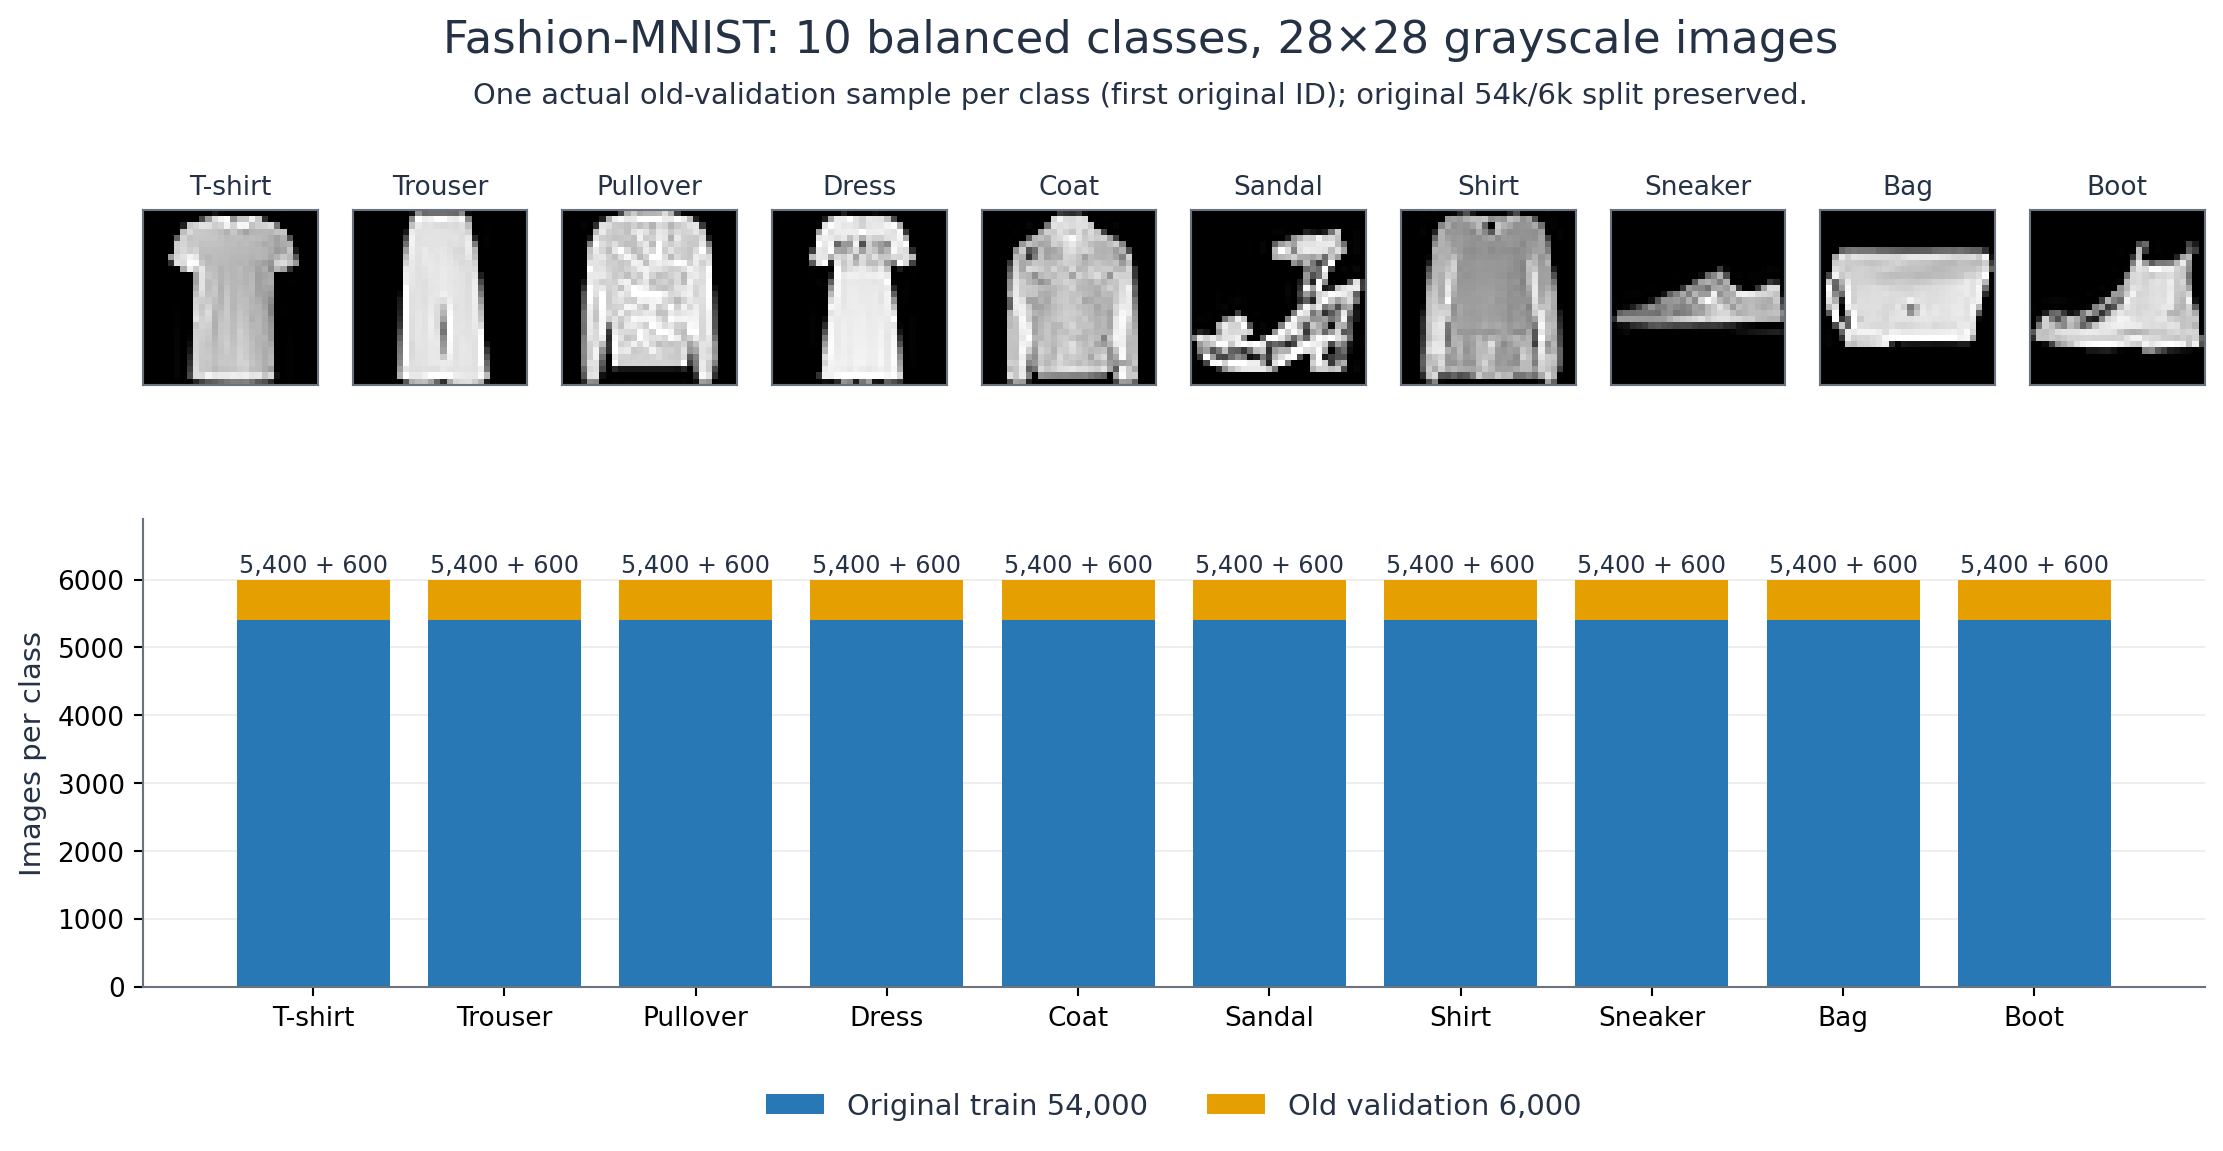
\includegraphics[width=\linewidth]{figures/dataset_overview.png}
\caption{Actual Fashion-MNIST samples and class counts from the preserved original split. The samples are the first old-validation ID in each true class; they are illustrative rather than randomly sampled.}
\label{fig:data}
\end{figure}
\subsection{Observed structure and ambiguity}
The data are balanced at the class level, but class difficulty is uneven. T-shirts, shirts, pullovers and coats often share grayscale outlines, whereas footwear and bags have more distinctive silhouettes in the displayed samples. Accuracy and macro-F1 are therefore complemented by class-level confusion rates. The sample grid motivates this analysis; the full predictions quantify its frequency.

At $28\times28$ pixels, color and fine texture are unavailable. Local edges and spatial arrangement motivate the CNN representation, while row and patch representations test alternative ways to encode context. Ambiguous thumbnails are retained with the supplied labels; visual ambiguity alone is insufficient evidence for relabeling.

\subsection{Input pipeline}
\begin{center}\small
\fbox{IDX images/labels}\ $\longrightarrow$\ \fbox{Saved split IDs}\ $\longrightarrow$\ \fbox{Float32 image tensors}\\[3mm]
\fbox{One of five models}\ $\longrightarrow$\ \fbox{Ten logits}\ $\longrightarrow$\ \fbox{CE for training; argmax for labels}
\end{center}
\texttt{ToTensor} converts unsigned pixel values from $[0,255]$ to float32 values in $[0,1]$. A batch has shape $B\times1\times28\times28$ and integer targets have shape $B$. The classification loss receives logits directly. Softmax is used conceptually to interpret class probabilities, not inserted before cross-entropy.

The recorded studies use no augmentation, channel-wise standardization, oversampling or pretrained features. A seeded generator shuffles training batches; validation uses a fixed order. Both loaders retain the short final batch.

During training, each minibatch performs gradient reset, forward propagation, cross-entropy evaluation, backpropagation, gradient-norm clipping and an optimizer update. Validation runs in evaluation mode with gradients disabled and does not update parameters. Epoch CE is sample-weighted,
\[
\mathrm{CE}_{\mathrm{epoch}}=\frac{\sum_b n_b\,\mathrm{CE}_b}{\sum_b n_b},
\]
so a short final batch has its correct contribution. Accuracy and macro-F1 are computed from the complete epoch confusion matrix, equivalently all epoch predictions, rather than averaging minibatch F1 values. Saved IDs connect those predictions to the original dataset images.

\bigskip
\section{Evaluation design}
\subsection{Preserved and nested partitions}
The original split uses split seed 42 and is stratified. Its sample IDs are retained throughout all studies. The final search creates one additional stratified split inside the original 54,000 training IDs, using inner split seed 20261022. All families use identical IDs at a given phase.

\begin{center}
\small
\begin{tabular}{lrrl}
\toprule
Partition & Images & Images/class & Role in final study \\
\midrule
Original train & 54,000 & 5,400 & Parent set for search; final training \\
Old validation & 6,000 & 600 & Final checkpoint selection \\
Inner train & 48,600 & 4,860 & Discovery and confirmation training \\
Inner validation & 5,400 & 540 & Recipe and checkpoint selection \\
Official test & 10,000 & 1,000 & Historical frozen results only \\
\bottomrule
\end{tabular}
\end{center}
Inner train and inner validation are disjoint and together recover the original training set. Neither contains old-validation IDs. Final training uses the original 54,000 images, with old validation still excluded from gradient updates. Each fit starts from a fresh seeded initialization. This keeps the inner-validation images outside the weight-update history of every search candidate.

\subsection{Metrics and checkpoint rules}
For a validation set of $N$ images, accuracy is $N^{-1}\sum_i\mathbf{1}[\hat y_i=y_i]$. For class $k$,
\[
F_{1,k}=\frac{2TP_k}{2TP_k+FP_k+FN_k},\qquad
F_{1,\mathrm{macro}}=\frac{1}{10}\sum_{k=0}^{9}F_{1,k}.
\]
Cross-entropy is $\mathrm{CE}=-N^{-1}\sum_i\log p_\theta(y_i\mid x_i)$. It is sensitive to the probability assigned to the true label; accuracy and macro-F1 depend on predicted classes. A later checkpoint may therefore improve F1 while worsening CE.

The original and intermediate studies retain the minimum-validation-CE checkpoint, taking the earliest epoch on an exact tie. Final OPT3 uses maximum validation macro-F1; exact F1 ties prefer lower CE, followed by the earlier epoch. These rules apply to every family within their respective study. Best-CE checkpoints are also retained as a secondary diagnostic. The OPT3 rule was fixed before the search began; the later study remains exploratory because the earlier test results were already known.

\subsection{Meaning of the reported variation}
For final seeds $s\in\{42,43,44\}$, the report gives the arithmetic mean and sample standard deviation, with denominator $n-1$. These quantify training-seed variation conditional on the fixed, selected validation set. Image-sampling uncertainty, split variation and deployment shift are outside this SD; the three runs are used descriptively rather than as a significance test.

\clearpage
\part{Models and optimization}
\section{Five model families}
\subsection{Architecture and parameter summary}
All models output $B\times10$ logits. Architecture sizes are held fixed in the search. Dropout changes stochastic regularization without adding parameters; schedule changes do not add parameters either.

\begin{center}
\small
\begin{tabular}{llr}
\toprule
Family & Main representation & Trainable parameters \\
\midrule
Linear & $784\rightarrow10$ & 7,850 \\
MLP & $784\rightarrow256\rightarrow10$ & 203,530 \\
CNN & 3 convolutions, channels $32/64/128$ & 93,962 \\
GRU & 28 steps, input 28, hidden 128 & 61,962 \\
Transformer & 49 patches, width 128, 2 layers & 274,954 \\
\bottomrule
\end{tabular}
\end{center}
\subsection{Linear classifier}
The image is flattened to 784 features and mapped by $z=Wx+b$ to ten logits. The parameter count is $784\cdot10+10=7,850$. Its decision boundaries are linear in pixel space, providing a low-cost reference for the value of nonlinear and spatial representations.

\subsection{MLP}
The MLP applies a 256-unit affine layer, ReLU and a ten-unit output layer:
\[
z=W_2\,\mathrm{ReLU}(W_1\,\mathrm{vec}(x)+b_1)+b_2.
\]
Its parameter count is $(784\cdot256+256)+(256\cdot10+10)=203,530$. ReLU makes the mapping nonlinear, but flattening removes an explicit local spatial bias. The final selected C7 recipe applies dropout $p=0.2$ to the hidden representation before the output layer.

\subsection{Custom CNN}
Three $3\times3$ convolutions use stride 1 and padding 1. ReLU follows each convolution. The first two blocks include $2\times2$ max pooling. The spatial shapes are
\[
\begin{split}
B\times1\times28\times28\rightarrow B\times32\times28\times28
\rightarrow B\times32\times14\times14\\
\rightarrow B\times64\times14\times14\rightarrow B\times64\times7\times7
\rightarrow B\times128\times7\times7.
\end{split}
\]
Global average pooling produces $B\times128$, followed by dropout and a ten-unit head. Convolutions contribute 320, 18,496 and 73,856 parameters; the head contributes 1,290, for 93,962 total. Local receptive fields and shared filters reduce the number of parameters needed to detect repeated spatial patterns. Pooling and global averaging reduce spatial detail while providing some tolerance to position changes. C5 retains the architecture and uses head dropout 0.3.

\clearpage
\subsection{Row-wise GRU}
Each image is a sequence of 28 rows, each containing 28 pixel values. The input becomes $B\times28\times28$. A one-layer, unidirectional GRU with hidden size 128 returns a final hidden state $h_{28}\in\mathbb{R}^{B\times128}$, followed by a linear classifier. The update gate controls how much of the previous hidden state is retained, while the reset gate controls its contribution to the candidate state \cite{gru}. In the PyTorch implementation,
\[
\begin{aligned}
r_t&=\sigma(W_{ir}x_t+b_{ir}+W_{hr}h_{t-1}+b_{hr}),\\
z_t&=\sigma(W_{iz}x_t+b_{iz}+W_{hz}h_{t-1}+b_{hz}),\\
\widetilde h_t&=\tanh\!\left(W_{in}x_t+b_{in}+r_t\odot(W_{hn}h_{t-1}+b_{hn})\right),\\
h_t&=(1-z_t)\odot\widetilde h_t+z_t\odot h_{t-1}.
\end{aligned}
\]
Here $x_t\in\mathbb R^{28}$ and $h_t,r_t,z_t\in\mathbb R^{128}$. The reset gate is applied after the hidden-state affine transform, matching the implemented library operation.\footnote{PyTorch 2.11 GRU definition: \url{https://docs.pytorch.org/docs/2.11/generated/torch.nn.GRU.html}.}

The row representation imposes an ordering on spatial data. It can summarize dependencies across image rows, but introduces directional bias and sequential computation. The matched row-versus-column ablation examines the effect of this ordering for the fixed architecture and training setup.

The parameter count is
\[
3(128)(28)+3(128)(128)+2(3)(128)+(128)(10)+10=61,962.
\]
For one recurrent layer, PyTorch's built-in GRU dropout between layers is inactive. The optimization implementation therefore provides explicit optional dropout on the final hidden state. The selected C1 recipe uses no external head dropout and retains the row representation.

\subsection{Patch Transformer}
A stride 4, kernel 4 convolution embeds non-overlapping patches. The $28\times28$ image yields $7\times7=49$ tokens, each of dimension 128. Learned position embeddings have shape $1\times49\times128$. Two encoder layers each use four attention heads, a 256-wide feed-forward block, ReLU, residual connections, layer normalization and dropout. Attention uses
\[
\mathrm{Attention}(Q,K,V)=\mathrm{softmax}\left(\frac{QK^\top}{\sqrt{d_k}}\right)V,
\qquad d_k=128/4=32.
\]
Within each head, $Q$, $K$ and $V$ are learned projections of the 49 position-enriched token features, each with shape $B\times49\times32$. Attention weights relate every query patch to all key patches; the weighted values form contextual token representations. Four head outputs are concatenated and projected back to width 128. After the two encoder layers, mean pooling over the 49 tokens, LayerNorm and a ten-class linear head produce the logits. The from-scratch encoder uses no class token and has 274,954 trainable parameters \cite{attention}.

The model can relate distant patches in one attention layer, but learns both feature extraction and spatial use from this small dataset. The search includes an independently initialized encoder probe because the legacy encoder layers begin with equal initial values while remaining distinct parameters. The selected C1 recipe retains legacy initialization and uses warmup plus cosine decay. The initialization probe is one candidate comparison within this search, rather than a general conclusion about encoder initialization.

\subsection{Training objective and optimizers}
All five families minimize hard-label cross-entropy on minibatches of 128. Gradient norm clipping uses threshold 1. Inputs and model parameters are float32, without mixed-precision scaling. Linear and MLP use Adam \cite{adam}; CNN, GRU and Transformer use AdamW \cite{adamw}. Optimizer type and model size remain fixed during the final search. Adam applies the configured decay within its gradient-based update, whereas AdamW decouples decay from the adaptive gradient step. Equal numeric coefficients therefore do not define identical regularization across these optimizer families.

\clearpage
\section{Optimization protocol}
\subsection{Question, search space and budget}
The final study asks whether training recipes improve within fixed model families. It uses a seeded, finite random search with controlled probes, rather than a full Cartesian grid or Bayesian adaptation. Optuna's RandomSampler is used to generate candidate values before observing objective scores \cite{optuna}. The candidate manifest is fixed, and no performance-based pruning replaces a weak candidate.

Linear has four candidates; the other four families each have eight. Candidate C0 is the original anchor. C1 changes the learning-rate schedule. C2 is a targeted probe for each nonlinear family: MLP/GRU external head dropout, CNN weight decay, or independent Transformer encoder initialization. Remaining candidates sample learning rate, weight decay and applicable dropout. Constant and scheduled learning rates are balanced within each family: 2/2 for Linear and 4/4 otherwise.

\begin{center}
\small
\begin{tabular}{lcll}
\toprule
Family & Candidates & LR range & Applicable dropout \\
\midrule
Linear & 4 & $3\times10^{-4}$--$3\times10^{-3}$ & None \\
MLP & 8 & $3\times10^{-4}$--$3\times10^{-3}$ & Hidden $0/0.1/0.2/0.3$ \\
CNN & 8 & $3\times10^{-4}$--$3\times10^{-3}$ & Head $0/0.1/0.2/0.3$ \\
GRU & 8 & $2\times10^{-4}$--$2\times10^{-3}$ & External head $0/0.1/0.2/0.3$ \\
Transformer & 8 & $10^{-4}$--$10^{-3}$ & Encoder $0.05/0.1/0.2/0.3$ \\
\bottomrule
\end{tabular}
\end{center}
Learning rates are sampled on a log scale. Sampled weight decay is one of $0,10^{-5},10^{-4},10^{-3}$. Controlled anchors/probes may retain the original value outside a sampled dropout range; the realized manifest is the authoritative candidate list in Appendix\ \ref{app:recipes}. There are only 36 discovery points across all five families, so the study cannot establish global hyperparameter optimality.

\subsection{Schedule and duration}
Every task completes 60 epochs. Constant schedules keep the configured learning rate. Cosine schedules decay to 5\% of the initial value; the Transformer scheduled probe combines five warmup epochs with cosine decay. The schedule follows optimizer-update counts and resumes from the saved update state. There are no cosine restarts. Inner fits use 380 updates per epoch, while final fits use 422, because $\lceil48,600/128\rceil=380$ and $\lceil54,000/128\rceil=422$.

The final stage trains on all 54,000 original training images for 60 epochs and retains the best checkpoint on the old 6,000-image validation set. Training completes the full budget; early stopping is not used. The selected epoch and the total executed epochs are recorded separately.

\clearpage
\subsection{Discovery, confirmation and final fits}
\begin{enumerate}
\item \textbf{Discovery:} The 36 candidates were trained with seed 101 on 48,600 inner-training images. Inner-validation macro-F1 selected the checkpoint within each fit and the best non-anchor challenger for each family. Scores within absolute $10^{-6}$ favored the lowest candidate ID.
\item \textbf{Additional confirmation:} C0 and the challenger for each family were trained with seed 202, giving 10 new fits. The decision used mean selected inner macro-F1 over seeds 101 and 202. A challenger was retained only when it exceeded the anchor mean by more than $10^{-6}$; otherwise C0 was retained.
\item \textbf{Final study:} The selected recipe for each family was trained from scratch with seeds 42,43 and 44 on the original 54,000 images. The old 6,000-image validation set selected the F1 checkpoint. These 15 completed fits form the final exploratory summary.
\end{enumerate}
The total is $36+10+15=61$ completed tasks and $61\cdot60=3,660$ model-epochs. Seed 101 is also used to discover the challenger. Thus, there is \emph{one fresh confirmation seed}, not two independently held-out confirmation runs. A positive mean across the two seeds is the locked decision rule, not a significance test.

\subsection{Controls and recovery}
Candidate configurations, effective hashes, source snapshots and split IDs bind a task to its intended recipe. Completed tasks preserve F1- and CE-selected checkpoints, predictions and a full 60-epoch history. Task transactions retain optimizer/RNG/loader state and checkpoint-selection state for recovery. A resumed task retains the same identity and random-state history; it is not counted as another independent seed.

All 61 recorded task attempts completed without an error. Software checks and experimental measurements are recorded separately.

\subsection{Selection scope}
The inner validation set is used for both checkpoint and recipe selection. The final old-validation set is also used to select final checkpoints. Its final score is consequently a selected validation estimate. The 15-fit OPT3 final stage did not train fresh C0 anchors alongside its selected recipes. That phase cannot isolate the effect of the recipe changes. Section~\ref{sec:matched-followup} supplies the later matched controls. Differences from older CE-selected baselines combine recipe changes, selection rules and potentially implementation/runtime effects.

\clearpage
\part{Results and interpretation}
\section{Original test study and intermediate evidence}
\subsection{Frozen official-test results}
Table\ \ref{tab:test} reports the original 20-epoch, seed 42 checkpoints evaluated on the 10,000-image official test. The checkpoints were selected by validation CE before the test evaluation. The later OPT3 checkpoints are evaluated only on validation, so this table remains the report's official-test comparison.
\begin{table}[H]\centering
\caption{Historical official-test results: original 20-epoch study, one training seed.}\label{tab:test}

\begin{center}
\small
\begin{tabular}{lrrrr}
\toprule
Model & Test accuracy(\%) & Test macro-F1(\%) & Parameters & Epoch \\
\midrule
Linear & 84.68 & 84.590 & 7,850 & 18 \\
MLP & 88.74 & 88.699 & 203,530 & 20 \\
CNN & 89.59 & 89.524 & 93,962 & 20 \\
GRU & 89.14 & 89.145 & 61,962 & 18 \\
Transformer & 88.94 & 88.829 & 274,954 & 20 \\
\bottomrule
\end{tabular}
\end{center}
\end{table}
The CNN has the highest recorded test accuracy, 89.59\%, exceeding the linear classifier by 4.91 percentage points. This is a fixed-budget, single-seed comparison. Its test estimates and the later selected-validation estimates answer different evaluation questions.

\subsection{Why extend beyond 20 epochs?}
The intermediate study uses seeds 42,43 and 44, best-CE selection, and a 60-epoch budget. For the CNN, best-through 60 minus best-through 20 improves validation accuracy by 2.417 percentage points on average, with sample SD 0.342. The MLP's best-CE F1 does not improve under that extension. More epochs therefore do not help every model equally.

The same intermediate study tests three ablations. Table\ \ref{tab:ablations} gives variant-minus-baseline F1 differences at 60 epochs. These are matched-seed validation comparisons under the earlier CE-selection protocol, separate from final OPT3.
\begin{table}[H]\centering\caption{Intermediate 60-epoch ablations; macro-F1 difference in percentage points, mean $\pm$sample SD over three matched seeds.}\label{tab:ablations}

\begin{center}
\small
\begin{tabular}{lr}
\toprule
Variant minus baseline & Macro-F1 delta(pp) \\
\midrule
cnn\_no\_dropout & $-0.069 \pm 0.155$ \\
gru\_columns & $-0.570 \pm 0.216$ \\
transformer\_no\_position & $-3.903 \pm 0.148$ \\
\bottomrule
\end{tabular}
\end{center}
\end{table}
CNN dropout removal has mixed-seed effects. Column scanning lowers GRU F1 on all three seeds. Removing Transformer positions also removes 6,272 parameters, so this probe changes capacity as well as position information.

\clearpage
\section{Final OPT3 validation results}
The selected recipes are Linear C1, MLP C7, CNN C5, GRU C1 and Transformer C1. All final fits use 60 epochs and the same preserved 54k/6k partition. Table\ \ref{tab:final} summarizes the F1-selected checkpoints over three training seeds. Accuracy/F1 are expressed as percentages; SD is in percentage points.
\begin{table}[H]\centering\caption{Final exploratory validation results; three seeds, sample SD.}\label{tab:final}

\begin{center}
\small
\begin{tabular}{lrrr}
\toprule
Model/recipe & Accuracy(\%) & Macro-F1(\%) & CE \\
\midrule
Linear / C1 & $86.856 \pm 0.010$ & $86.851 \pm 0.024$ & $0.3790 \pm 0.0009$ \\
MLP / C7 & $91.439 \pm 0.167$ & $91.448 \pm 0.153$ & $0.2630 \pm 0.0012$ \\
CNN / C5 & $93.278 \pm 0.059$ & $93.308 \pm 0.027$ & $0.1915 \pm 0.0003$ \\
GRU / C1 & $91.400 \pm 0.328$ & $91.367 \pm 0.376$ & $0.2748 \pm 0.0137$ \\
Transformer / C1 & $91.433 \pm 0.120$ & $91.431 \pm 0.096$ & $0.3092 \pm 0.0177$ \\
\bottomrule
\end{tabular}
\end{center}
\end{table}
\begin{figure}[H]
\centering
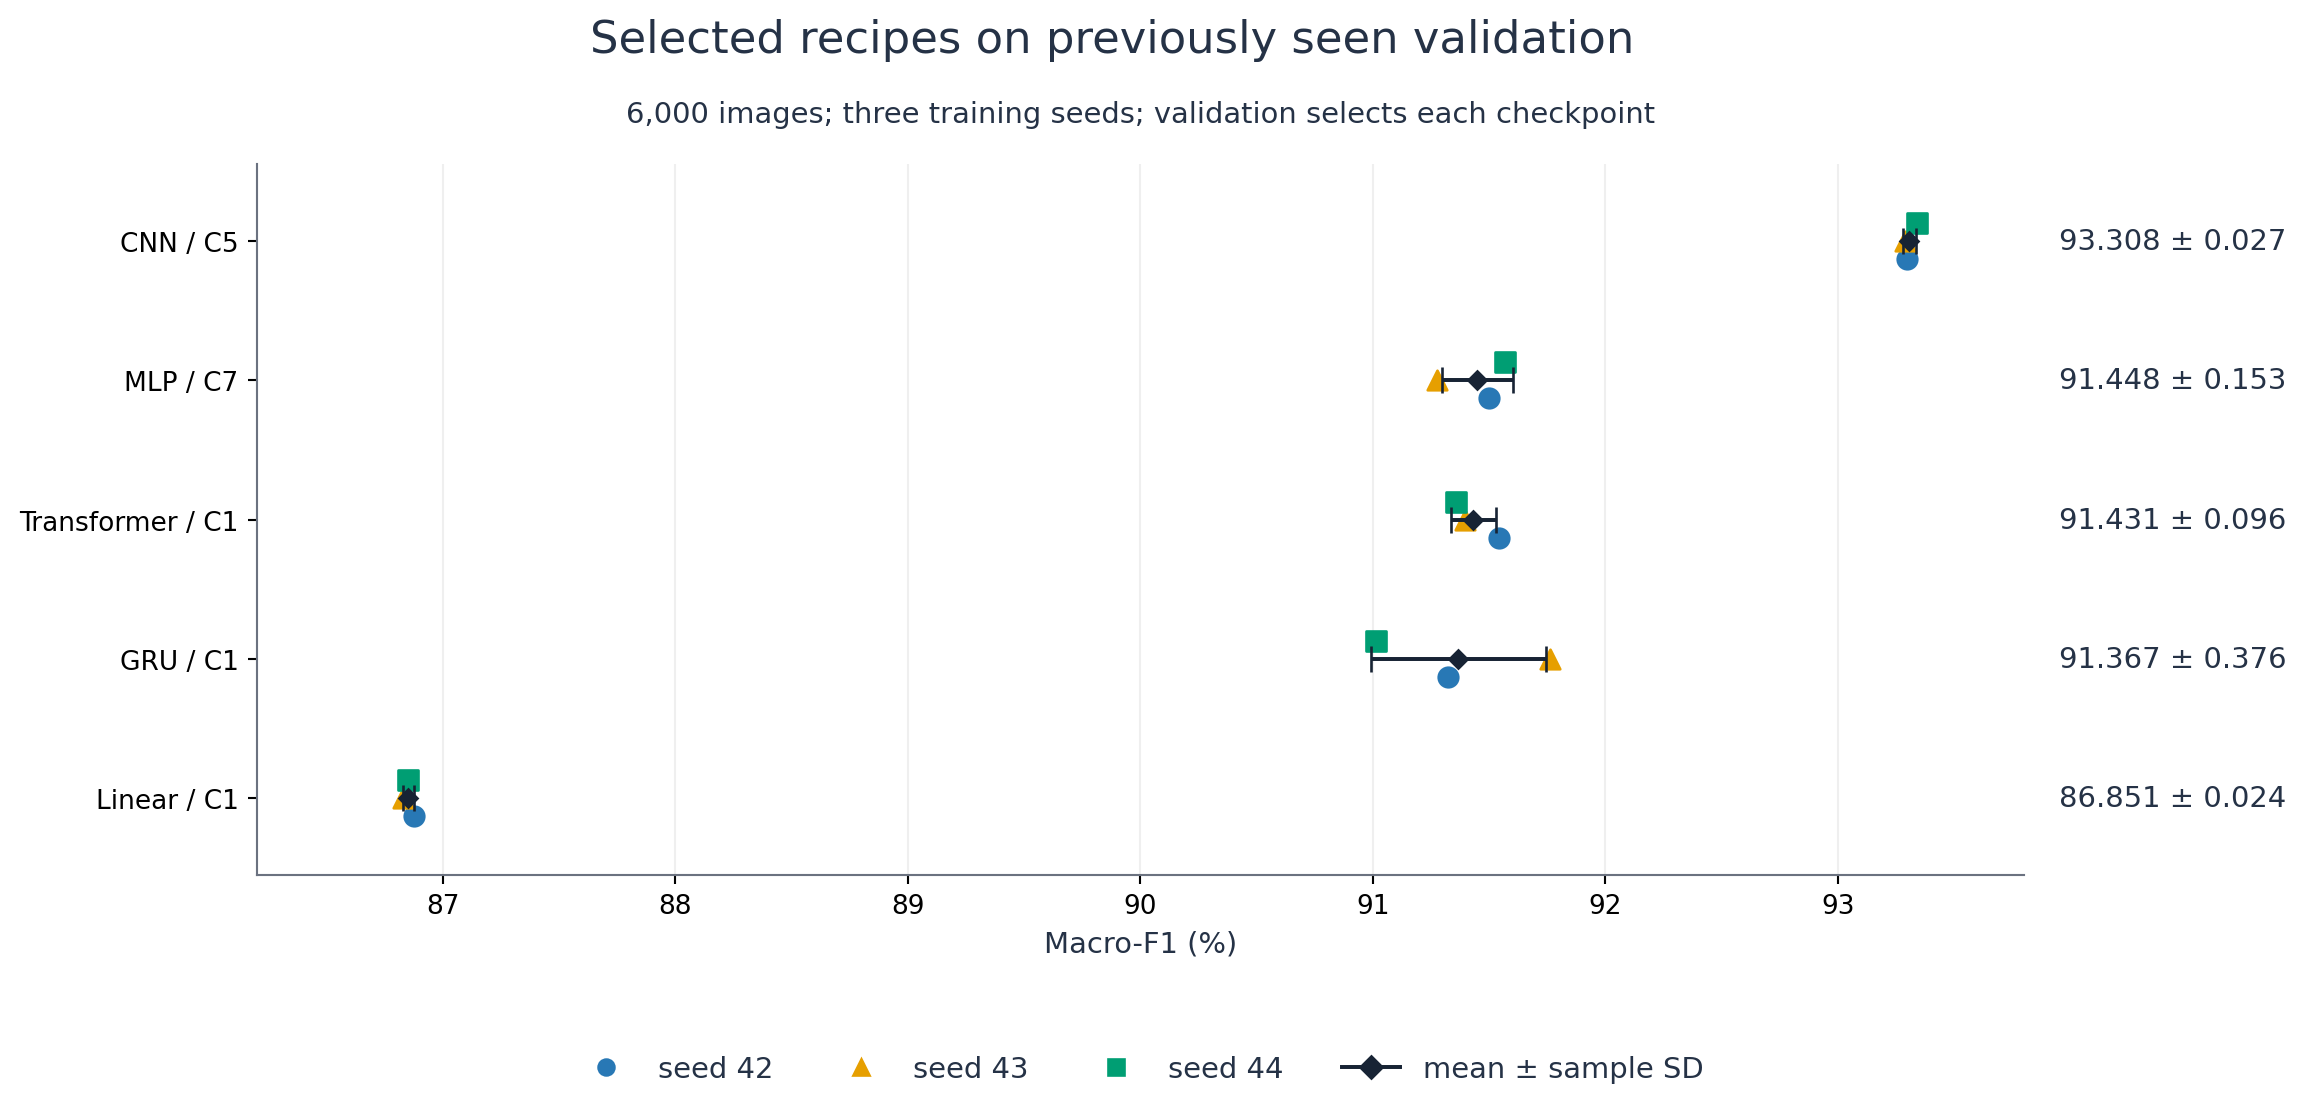
\includegraphics[width=\linewidth]{figures/final_f1_seeds.png}
\caption{Final old-validation macro-F1: individual seeds, mean and sample SD. Every point uses a checkpoint selected on these same 6,000 images. Small seed variation does not remove selection bias.}
\label{fig:final}
\end{figure}
CNN has the highest final validation mean. MLP and Transformer means are close, while GRU has greater seed variation. The ranking is conditional on Fashion-MNIST, the preserved split, the candidate space and the checkpoint-selection rule. The per-seed values are retained in Appendix\ \ref{app:seeds}.

\clearpage
\section{Search behavior and confirmation}
\subsection{Discovery coverage}

\begin{figure}[H]
\centering
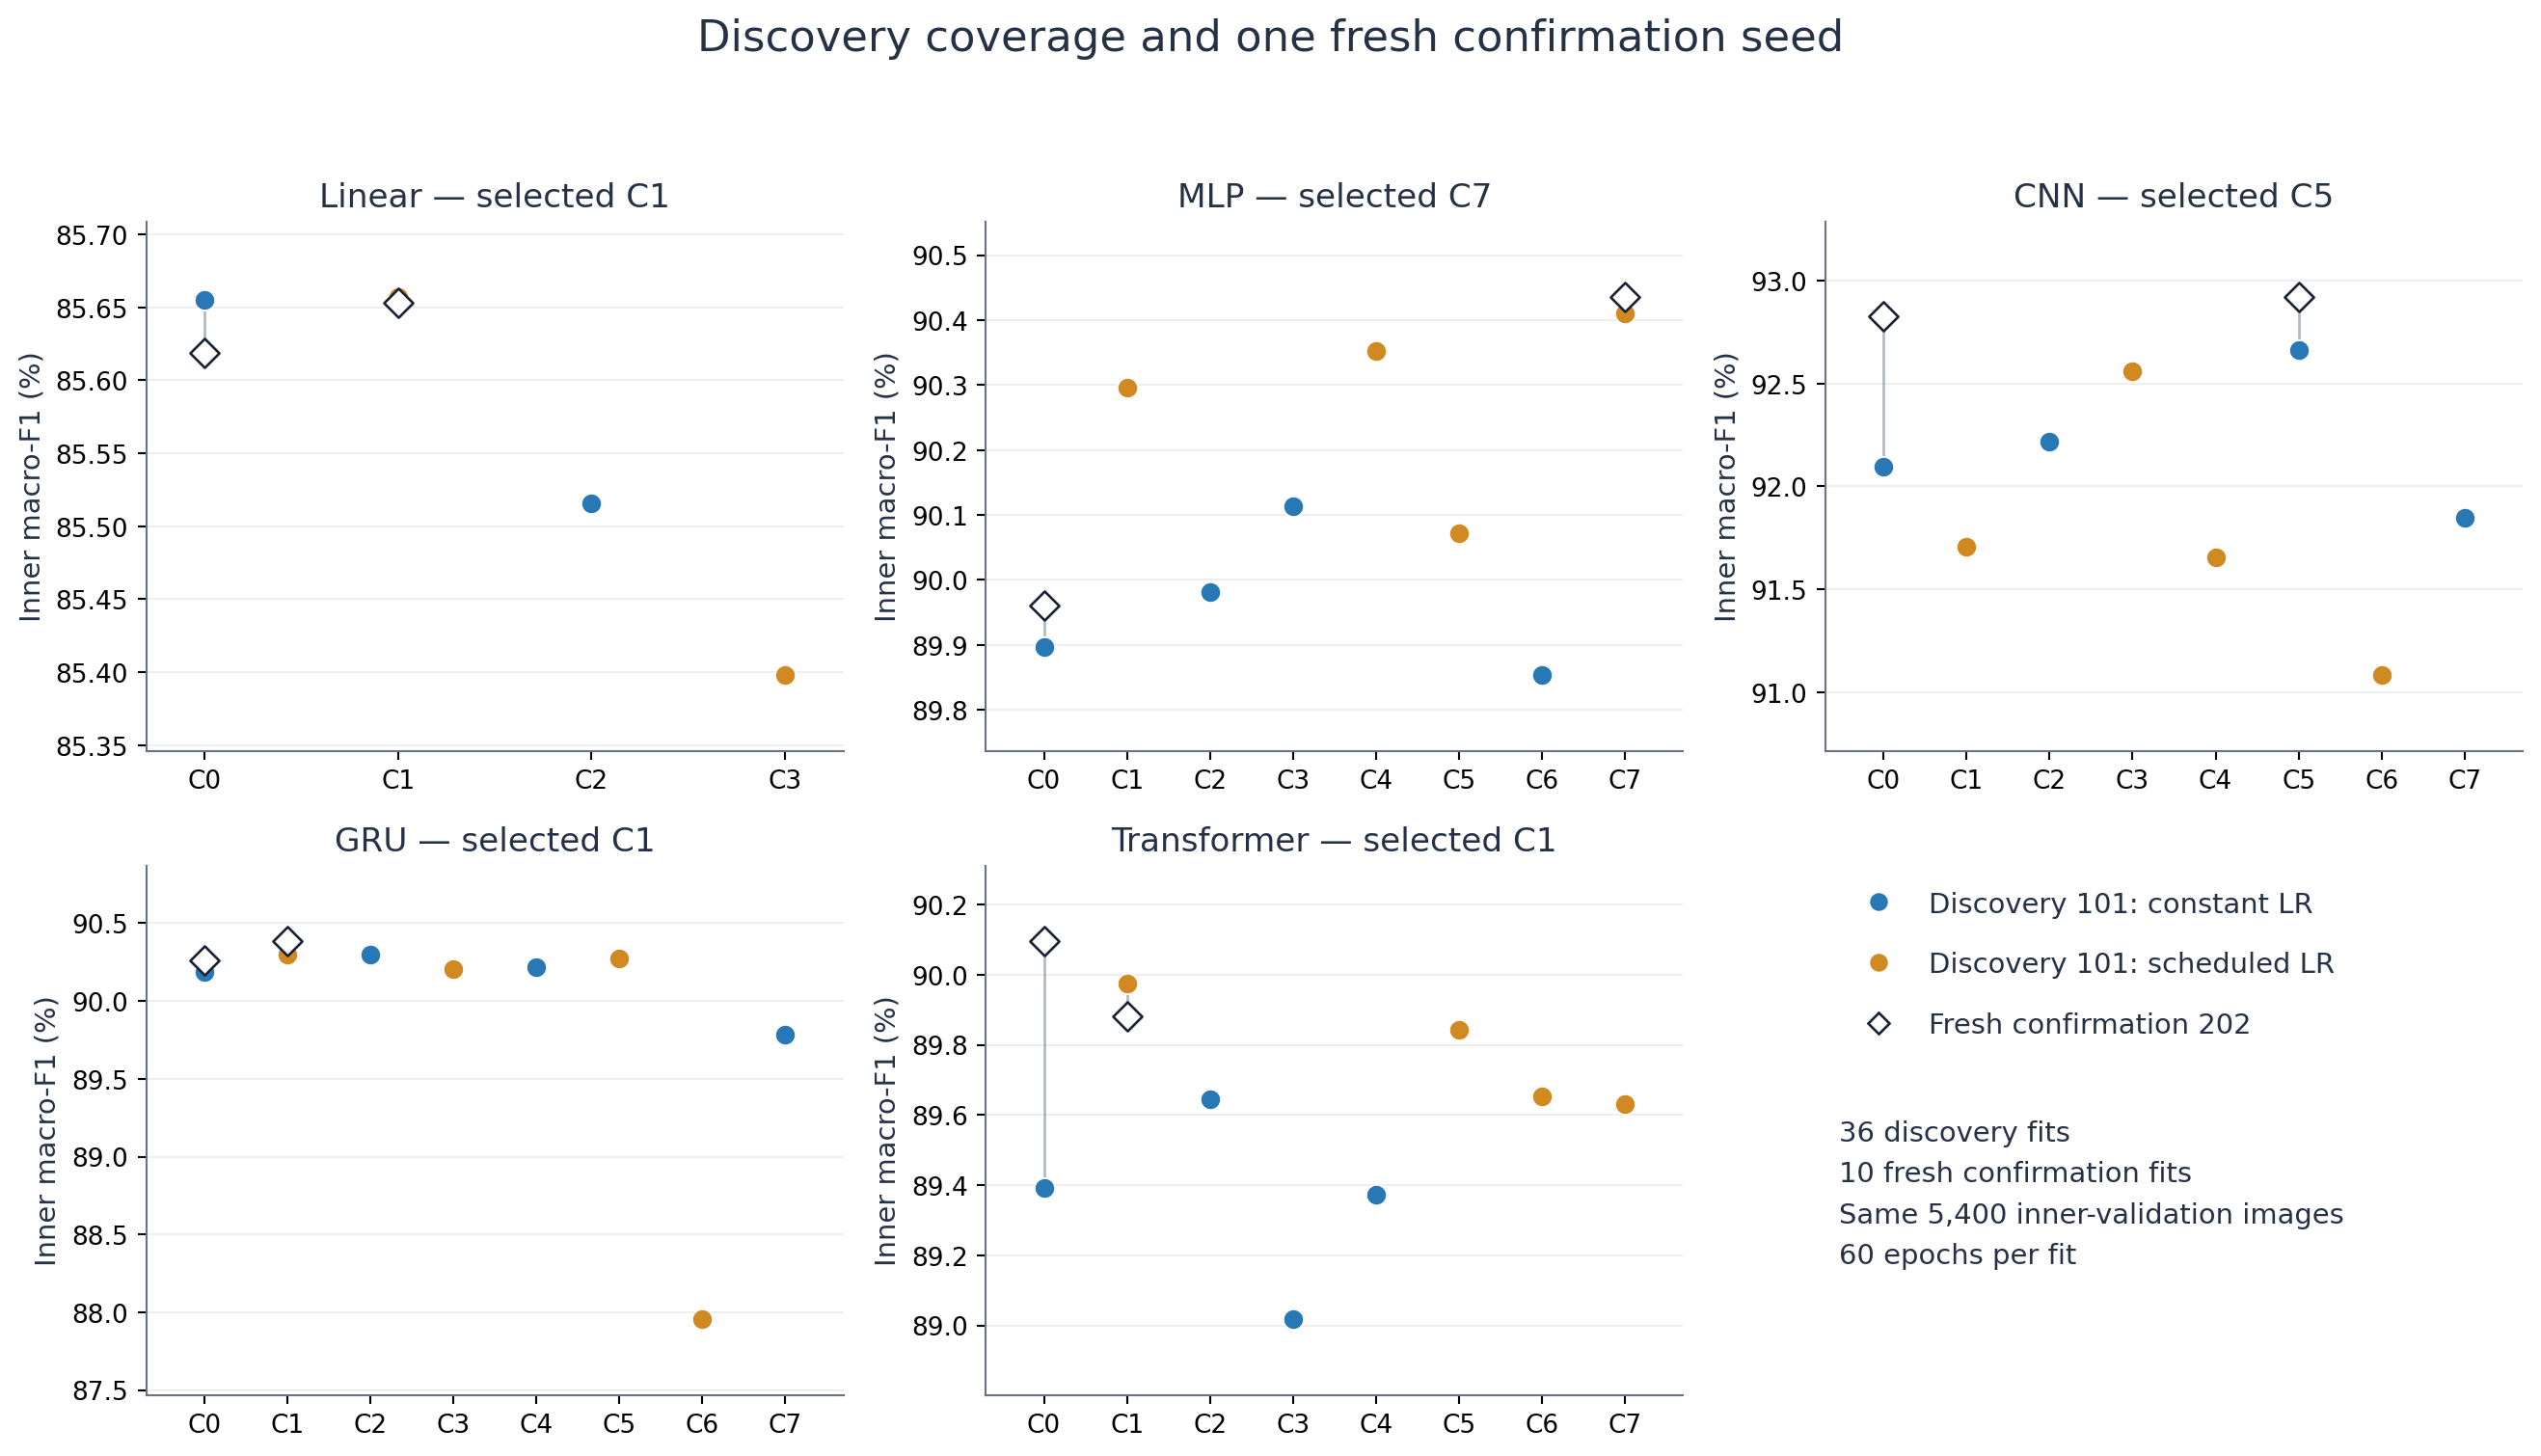
\includegraphics[width=\linewidth]{figures/discovery_confirmation.png}
\caption{All 36 discovery candidates and the 10 additional confirmation fits. Filled circles show seed 101; open diamonds show seed 202 for C0 and the selected challenger. Each panel uses the same inner-validation set but its own vertical scale.}
\label{fig:search}
\end{figure}
Several simple schedule probes survive the search: Linear, GRU and Transformer select C1. MLP selects C7, which combines cosine decay, learning rate approximately$1.010\times10^{-3}$, weight decay$10^{-5}$ and hidden dropout 0.2. CNN selects C5, a constant-LR recipe with learning rate approximately$1.438\times10^{-3}$, weight decay$10^{-4}$ and dropout 0.3.

These are recipe-level observations. The random candidates change multiple factors, so the MLP/CNN result does not identify a single responsible ingredient. The Transformer C1 probe combines warmup and cosine decay; its comparison does not isolate the effect of cosine alone. With eight candidates per nonlinear family, conclusions concern the realized recipes rather than global hyperparameter optima.

\clearpage
\subsection{Paired margins and one fresh seed}

\begin{figure}[H]
\centering
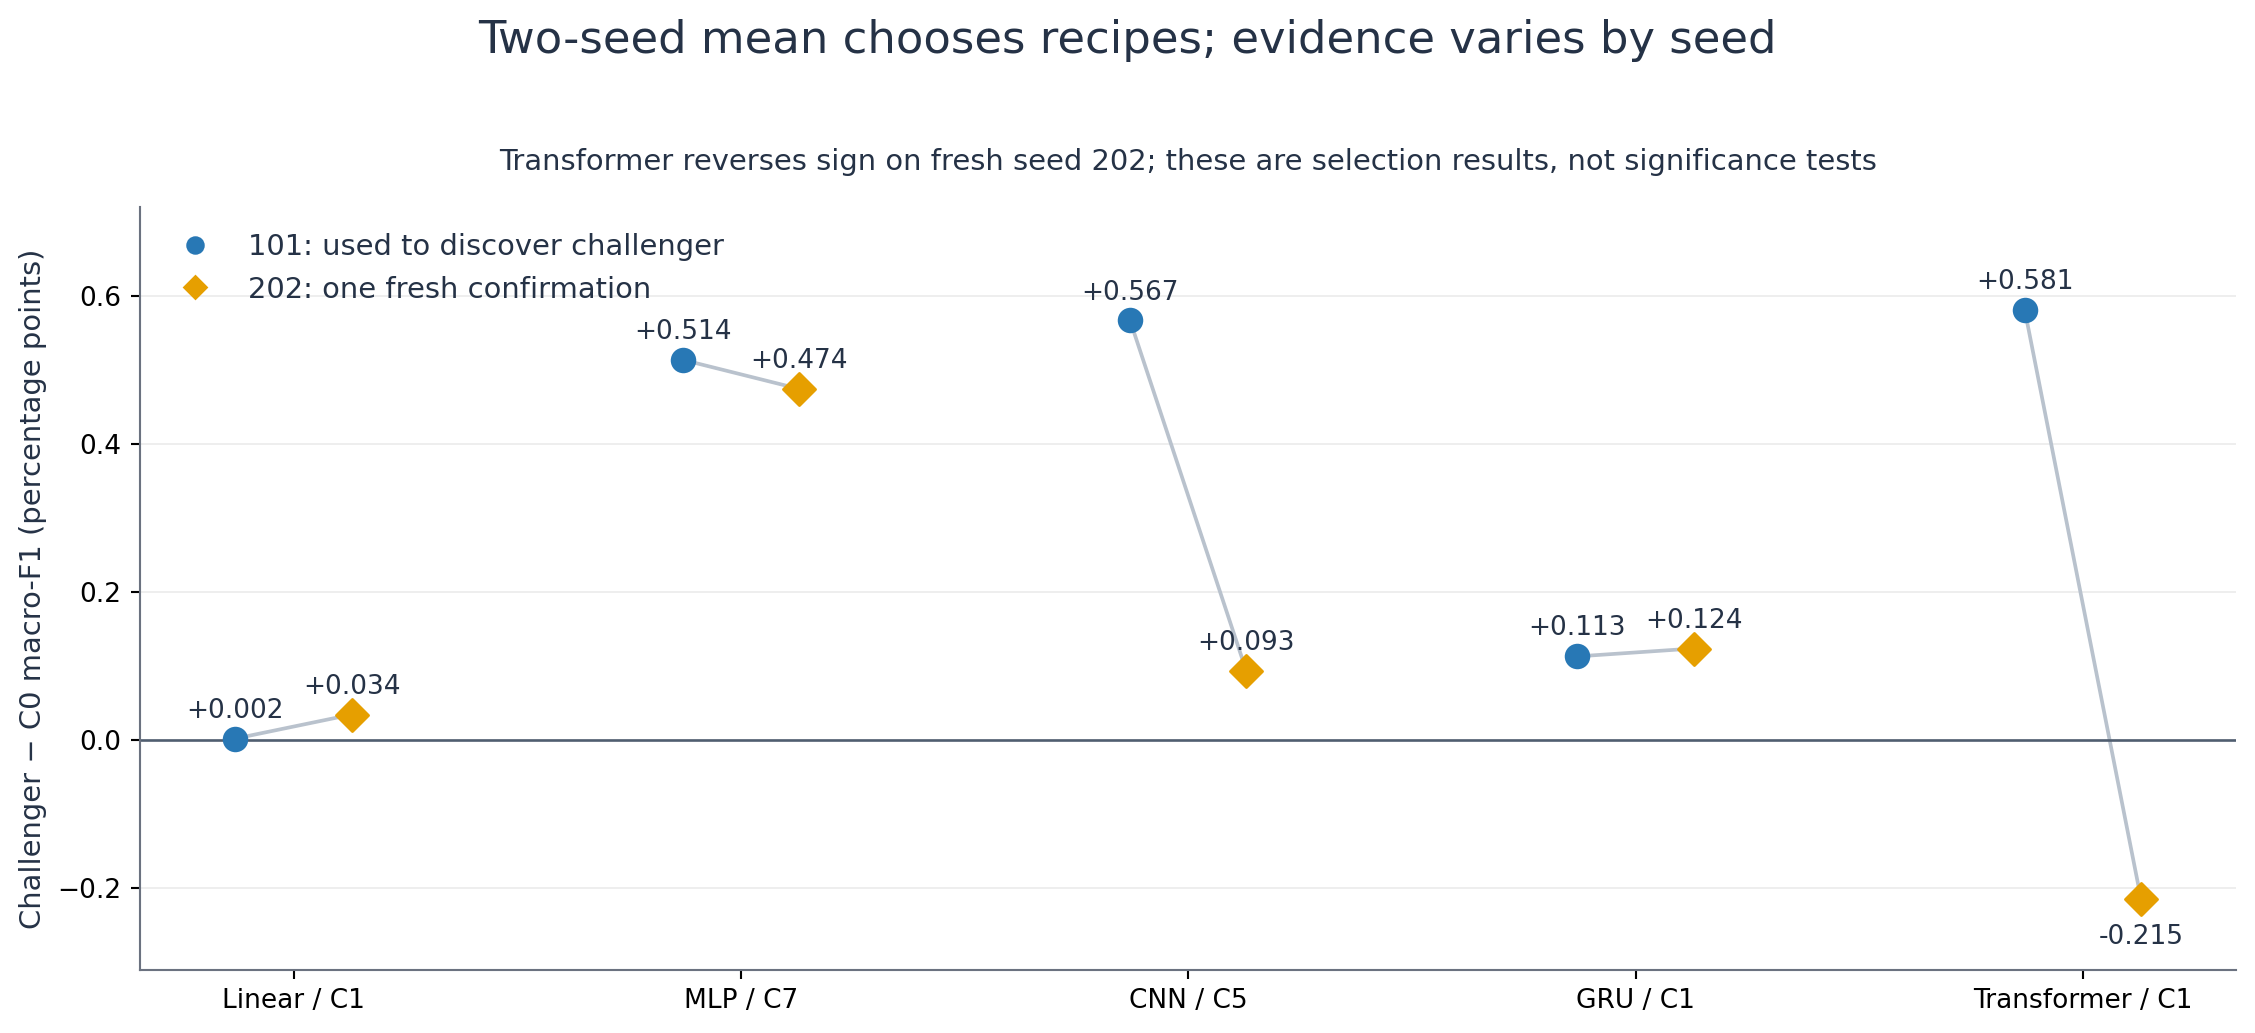
\includegraphics[width=\linewidth]{figures/paired_confirmation_deltas.png}
\caption{Challenger-minus-C0 F1 differences on the two matched inner seeds. Seed 101 already participated in discovery; seed 202 is the one fresh confirmation. Transformer changes sign, while the Linear difference is small.}
\label{fig:paired}
\end{figure}
\begin{center}
\small
\begin{tabular}{lcrrr}
\toprule
Family & Challenger & Seed 101(pp) & Seed 202(pp) & Mean(pp) \\
\midrule
Linear & C1 & +0.0020 & +0.0344 & +0.0182 \\
MLP & C7 & +0.5136 & +0.4743 & +0.4940 \\
CNN & C5 & +0.5668 & +0.0930 & +0.3299 \\
GRU & C1 & +0.1130 & +0.1236 & +0.1183 \\
Transformer & C1 & +0.5812 & -0.2146 & +0.1833 \\
\bottomrule
\end{tabular}
\end{center}
MLP C7 improves by about 0.514 and 0.474 percentage points on the two seeds. CNN C5 has a larger discovery gain than fresh-seed gain. Linear C1 clears the decision threshold but its mean gain is only about 0.018 percentage points. The Transformer gains 0.581 points on seed 101 and loses 0.215 on seed 202. Its positive two-seed mean selects C1 under the locked rule, while the mixed signs limit confidence that the change consistently improves this family.

The discovery seed's selected challenger is subject to selection bias because it was chosen from several alternatives. The second seed reduces dependence on a single lucky fit, but does not create a new data split. The individual paired margins expose the consistency and scale of the selection evidence.

\clearpage
\section{Learning dynamics and checkpoint choice}

\begin{figure}[H]
\centering
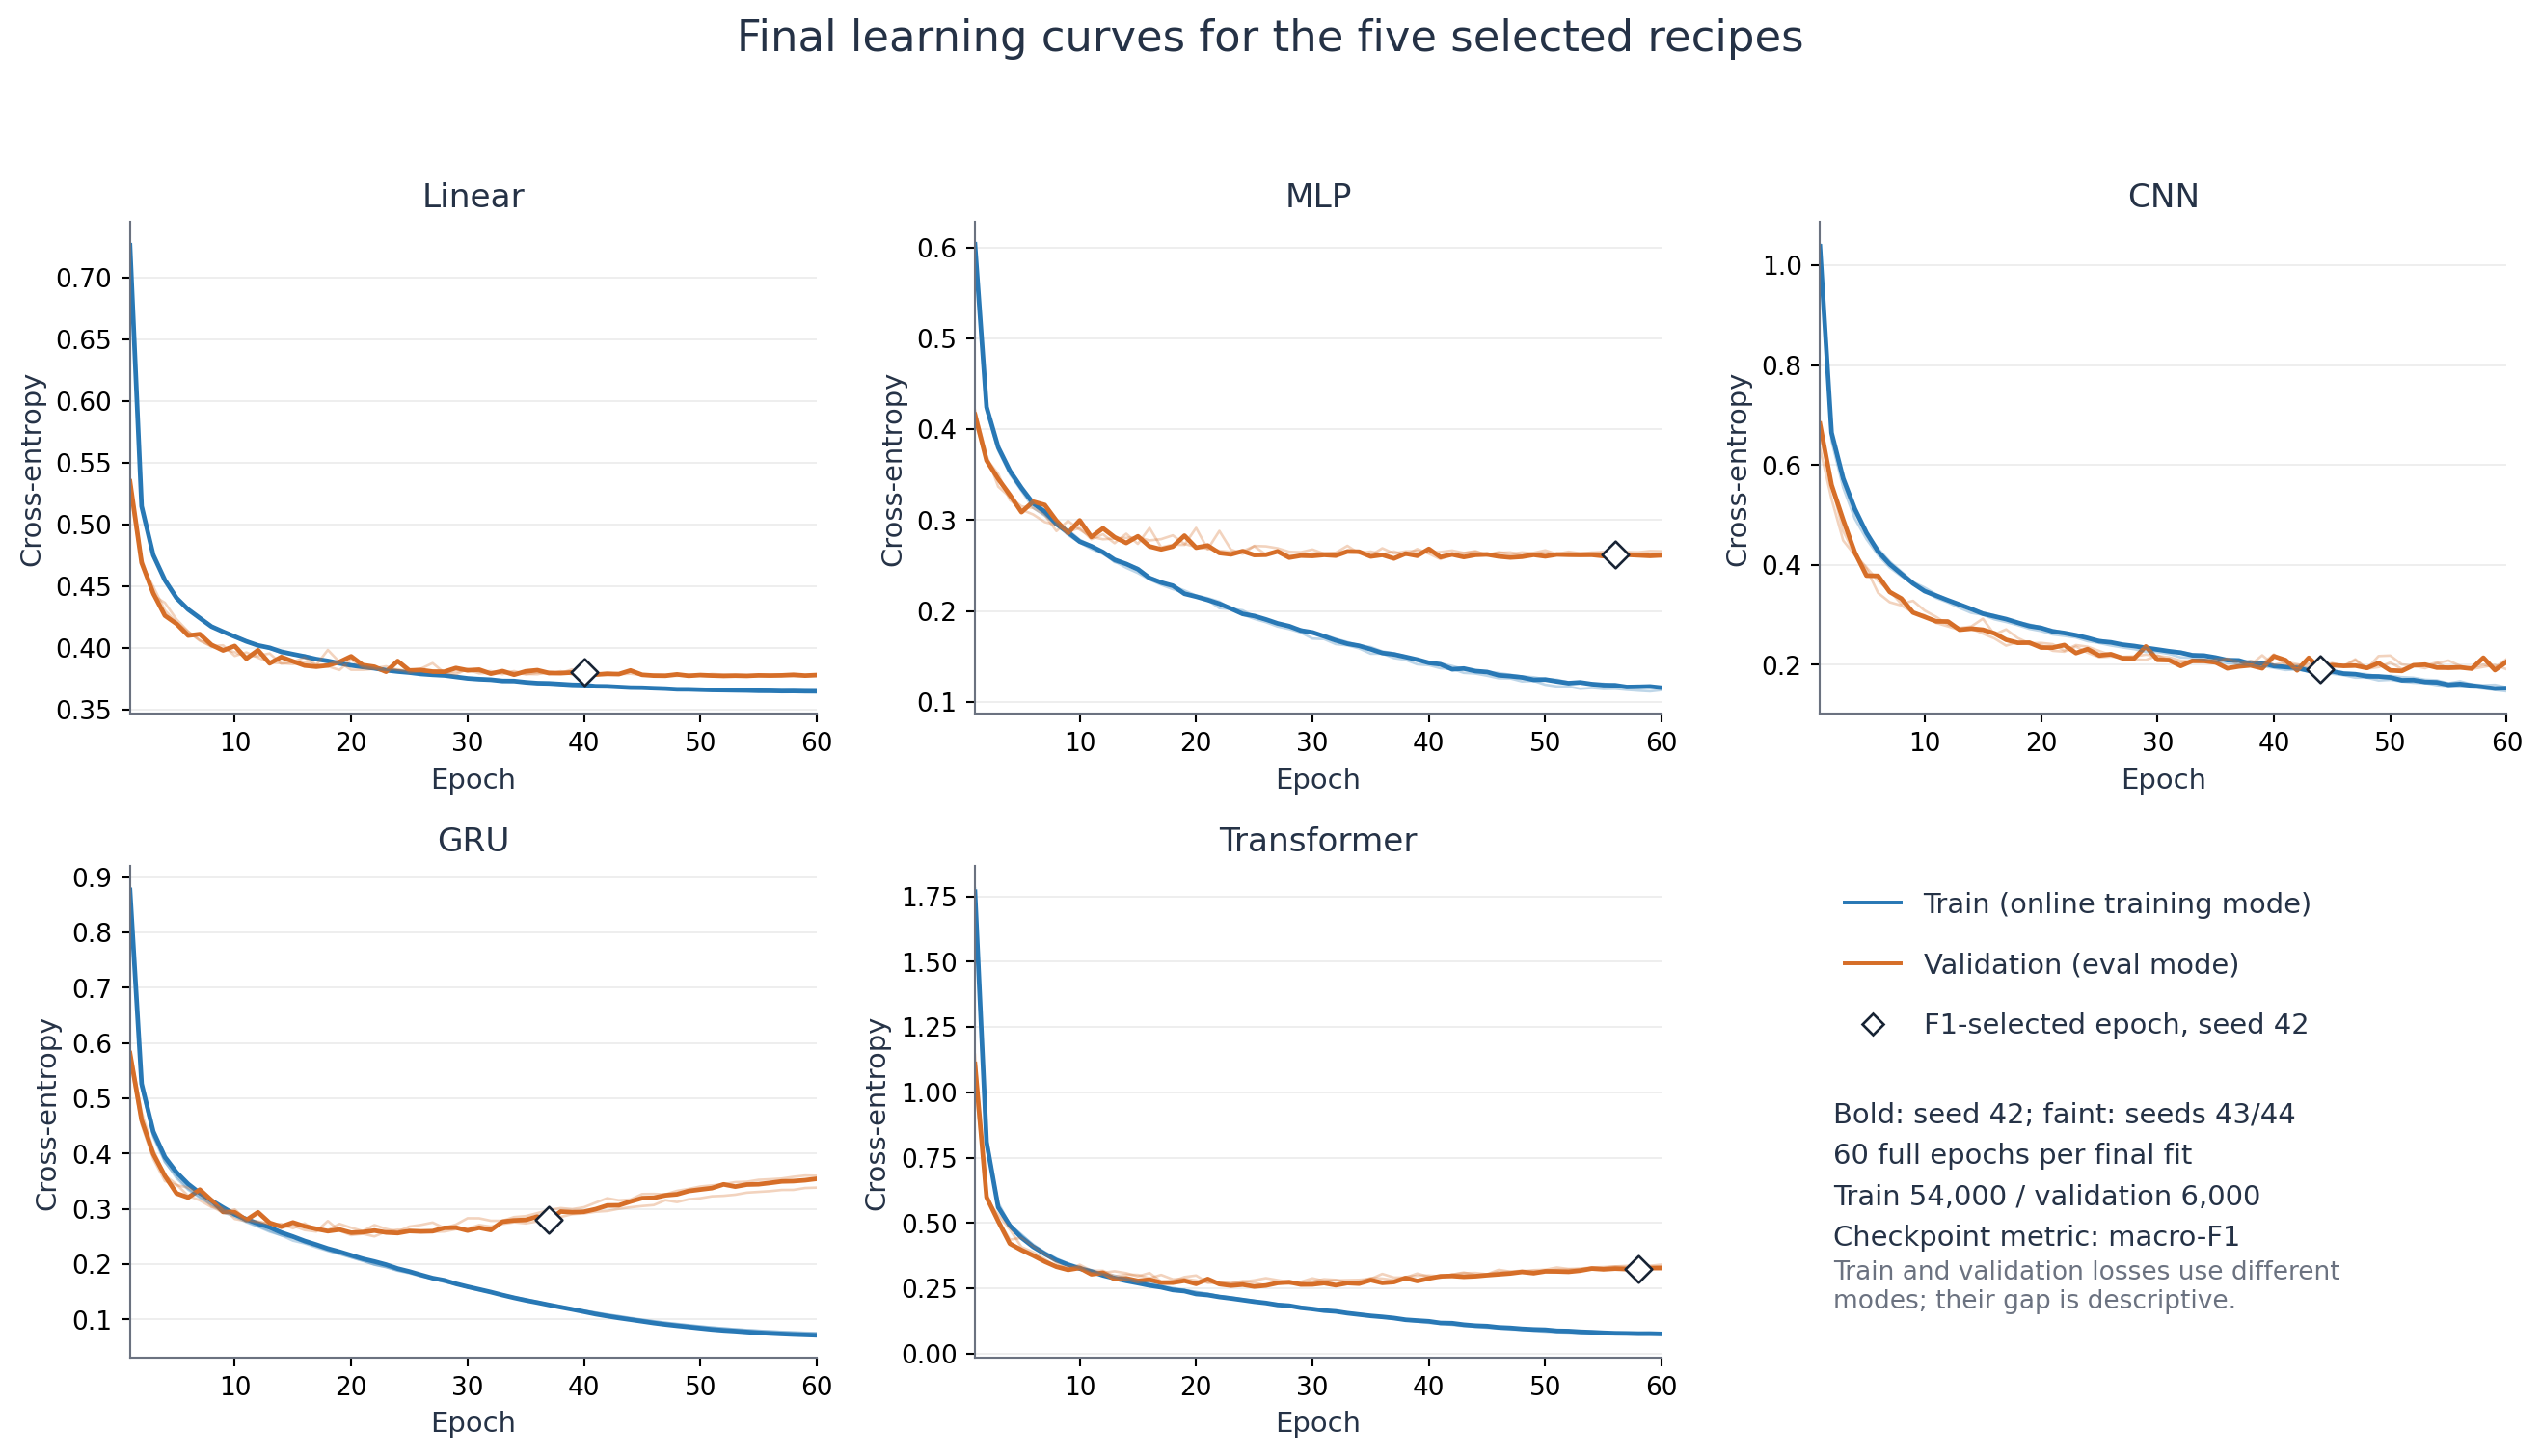
\includegraphics[width=\linewidth]{figures/learning_curves.png}
\caption{Actual unsmoothed final learning curves. Bold lines are seed 42; faint lines are seeds 43/44. Diamonds identify the seed 42 F1-selected epoch. Train loss is an online training-mode measure, whereas validation uses evaluation mode.}
\label{fig:curves}
\end{figure}
The CNN continues to learn useful representations late in training, although its validation CE fluctuates. MLP C7 reaches a comparatively flat validation-CE region while training loss continues downward. GRU and Transformer show increasing validation CE late in training even though some later epochs can still have competitive F1. CE deterioration diagnoses worsening probability loss, not necessarily worsening classification at every later epoch.

For CNN C5, seed 42, the F1 checkpoint is epoch 44: F1=0.932954 and CE=0.191585. The CE checkpoint is epoch 51: F1=0.932818 and CE=0.187897. Epoch 60 has F1=0.926353. Thus, choosing the last epoch would lose F1 in this particular fit, while minimum CE and maximum F1 select different valid checkpoints. The example demonstrates an objective trade-off along one trajectory: class-wise decision quality and true-label probability loss need not select the same epoch.

The train--validation gap cannot be interpreted as a perfectly matched measurement of generalization because train metrics use dropout and evolving weights during the epoch. Validation is measured after the epoch with dropout disabled. The upward validation-CE trend remains observable independently of that mode difference.

\clearpage
\section{Error analysis}
\subsection{CNN confusion structure}

\begin{figure}[H]
\centering
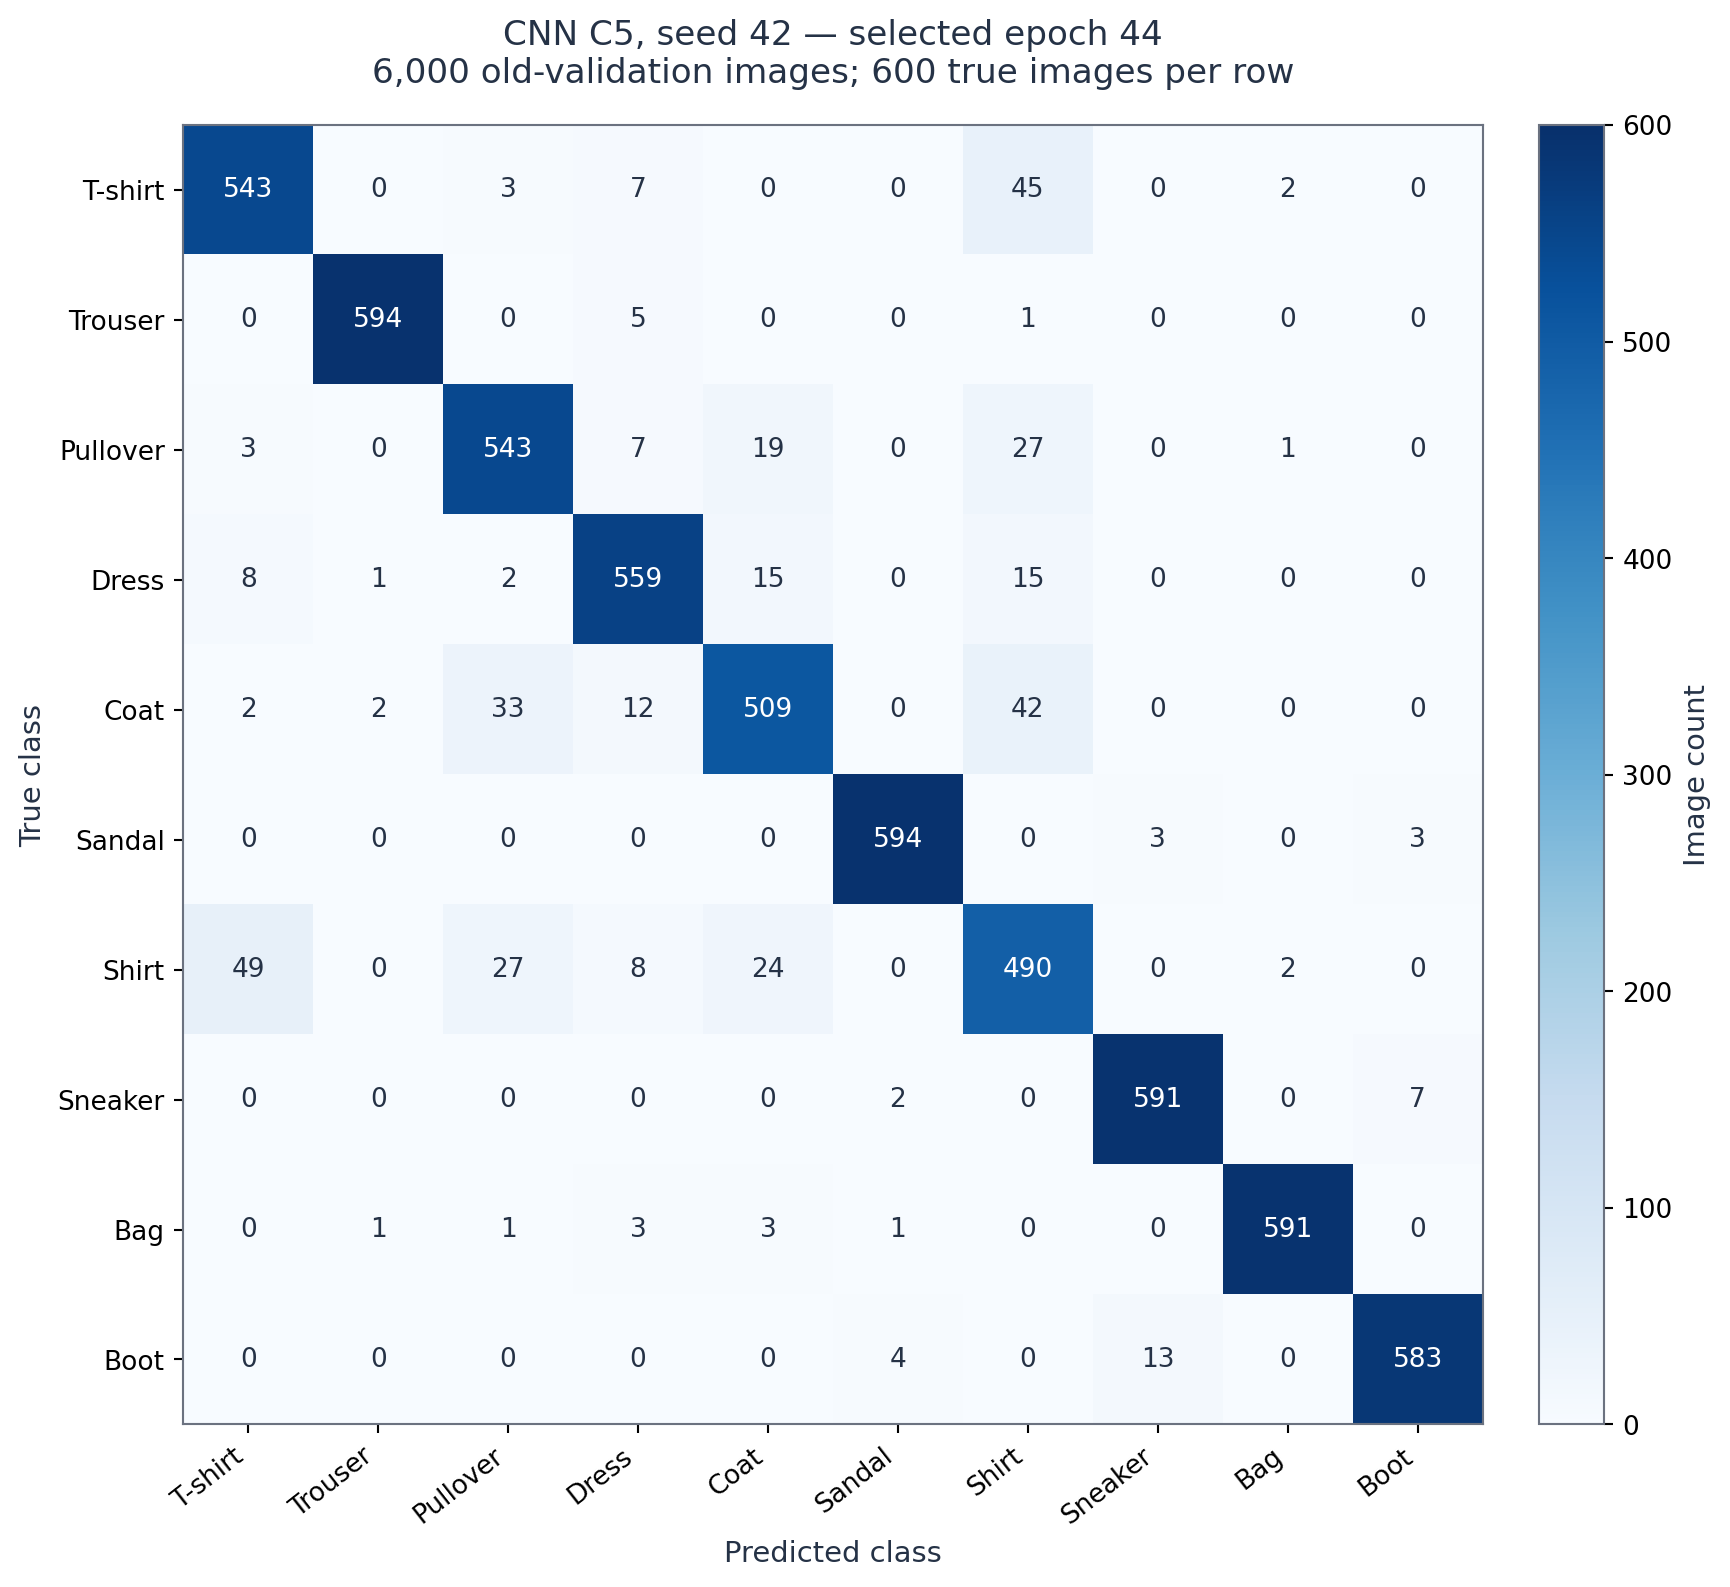
\includegraphics[width=0.84\linewidth]{figures/cnn_seed42_confusion.png}
\caption{CNN C5, seed 42, epoch 44, on old validation. Rows are true classes and columns are predicted classes. Each row contains 600 images; cells are integer prediction counts.}
\label{fig:confusion}
\end{figure}
The largest confusion is Shirt $\rightarrow$ T-shirt: 49/600 = 8.17\% of true shirts. T-shirt $\rightarrow$ Shirt: 45/600 = 7.50\%, and Coat $\rightarrow$ Shirt: 42/600 = 7.00\%. These rates use the true-class denominator, not all 6,000 images. Trouser and Sandal each have 594/600 correct predictions in this checkpoint, whereas Shirt has 490/600.

The errors are concentrated among upper-body garments rather than evenly spread across classes. A plausible explanation is overlapping shape and texture at low resolution. The matrix establishes the confusion pattern; the proposed visual mechanism remains an interpretation to check against examples or a controlled experiment.

\clearpage
\subsection{Concrete examples and class-level variation}

\begin{figure}[H]
\centering
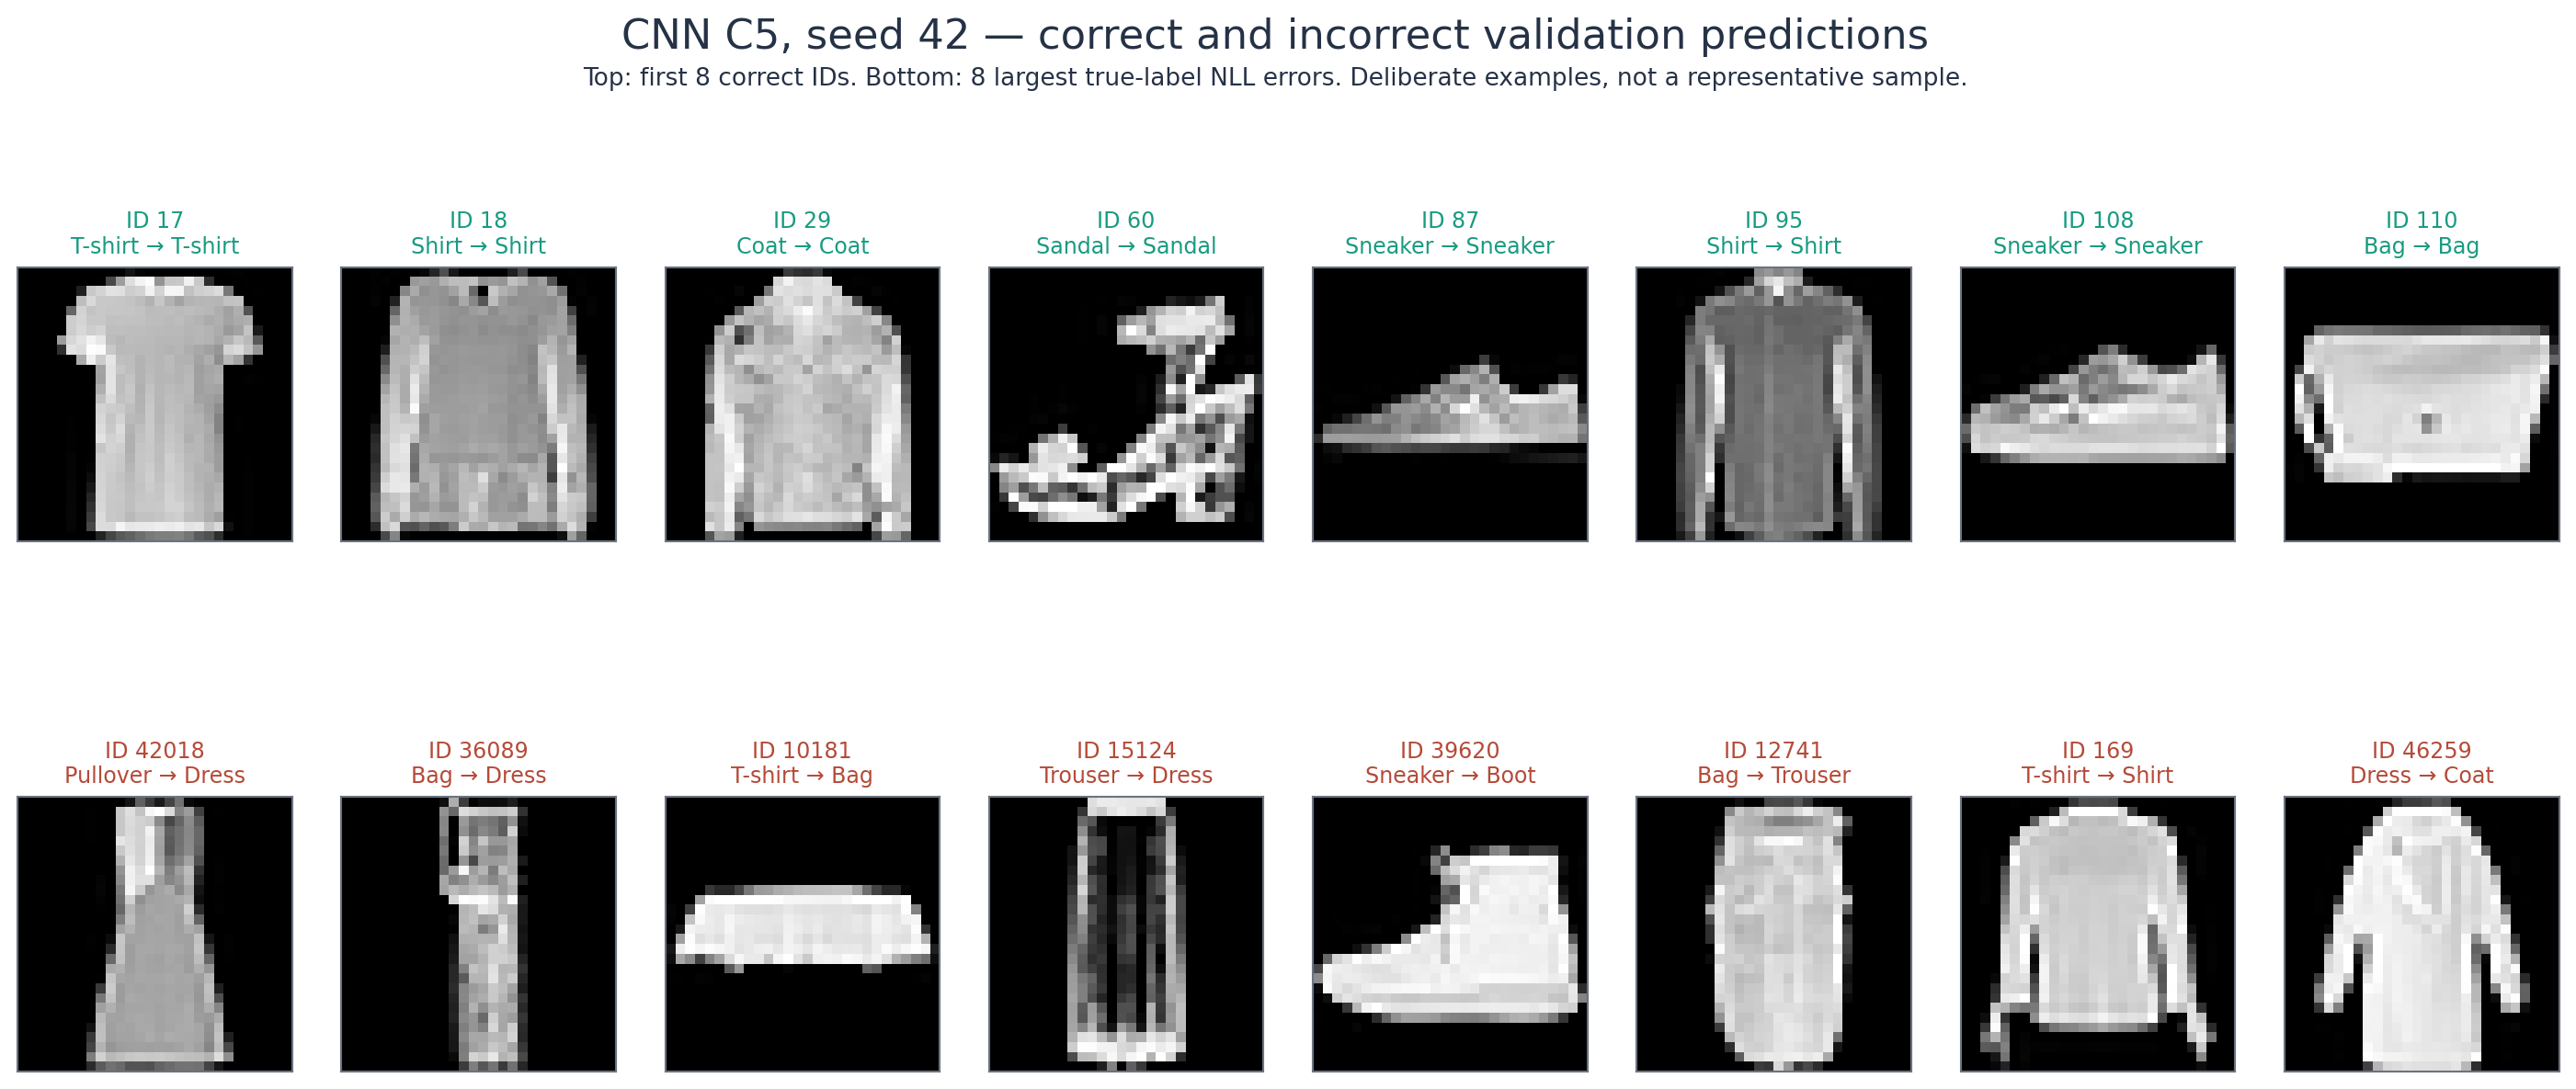
\includegraphics[width=\linewidth]{figures/cnn_seed42_examples.png}
\caption{Actual CNN C5 seed 42 predictions mapped back to official training-image IDs. Top: the first eight correct predictions by ID. Bottom: the eight errors with largest recorded true-label NLL. This deliberate selection illustrates failure cases and does not estimate their frequency.}
\label{fig:examples}
\end{figure}
Some selected errors have shapes that resemble the predicted class, including items labeled as bags or pullovers with unusual silhouettes. The supplied labels are retained. NLL ordering emphasizes errors to which the model assigns particularly unfavorable true-label probability, while the complete confusion matrix establishes the frequency of each error category.

The table below complements the single-seed image examples with CNN class F1 over all three final seeds. Its SD still describes training variation on the same validation images.

\begin{center}
\small
\begin{tabular}{lrr}
\toprule
Class & CNN class F1(\%) & Sample SD(pp) \\
\midrule
T-shirt/top & 90.12 & 0.59 \\
Trouser & 99.22 & 0.05 \\
Pullover & 89.53 & 0.29 \\
Dress & 93.01 & 0.08 \\
Coat & 87.61 & 0.57 \\
Sandal & 99.09 & 0.17 \\
Shirt & 80.15 & 0.43 \\
Sneaker & 97.70 & 0.26 \\
Bag & 98.78 & 0.05 \\
Ankle boot & 97.88 & 0.18 \\
\bottomrule
\end{tabular}
\end{center}
Shirt has the lowest mean class F1, about 80.15\%, despite the overall macro-F1 exceeding 93\%. The class-level results identify upper-body garment discrimination as the main remaining weakness. A targeted future comparison could test whether higher-resolution features or class-aware training improve these confusions while retaining the same evaluation protocol; those effects are not measured here.

\clearpage
\section{Efficiency and measured runtime}

\begin{figure}[H]
\centering
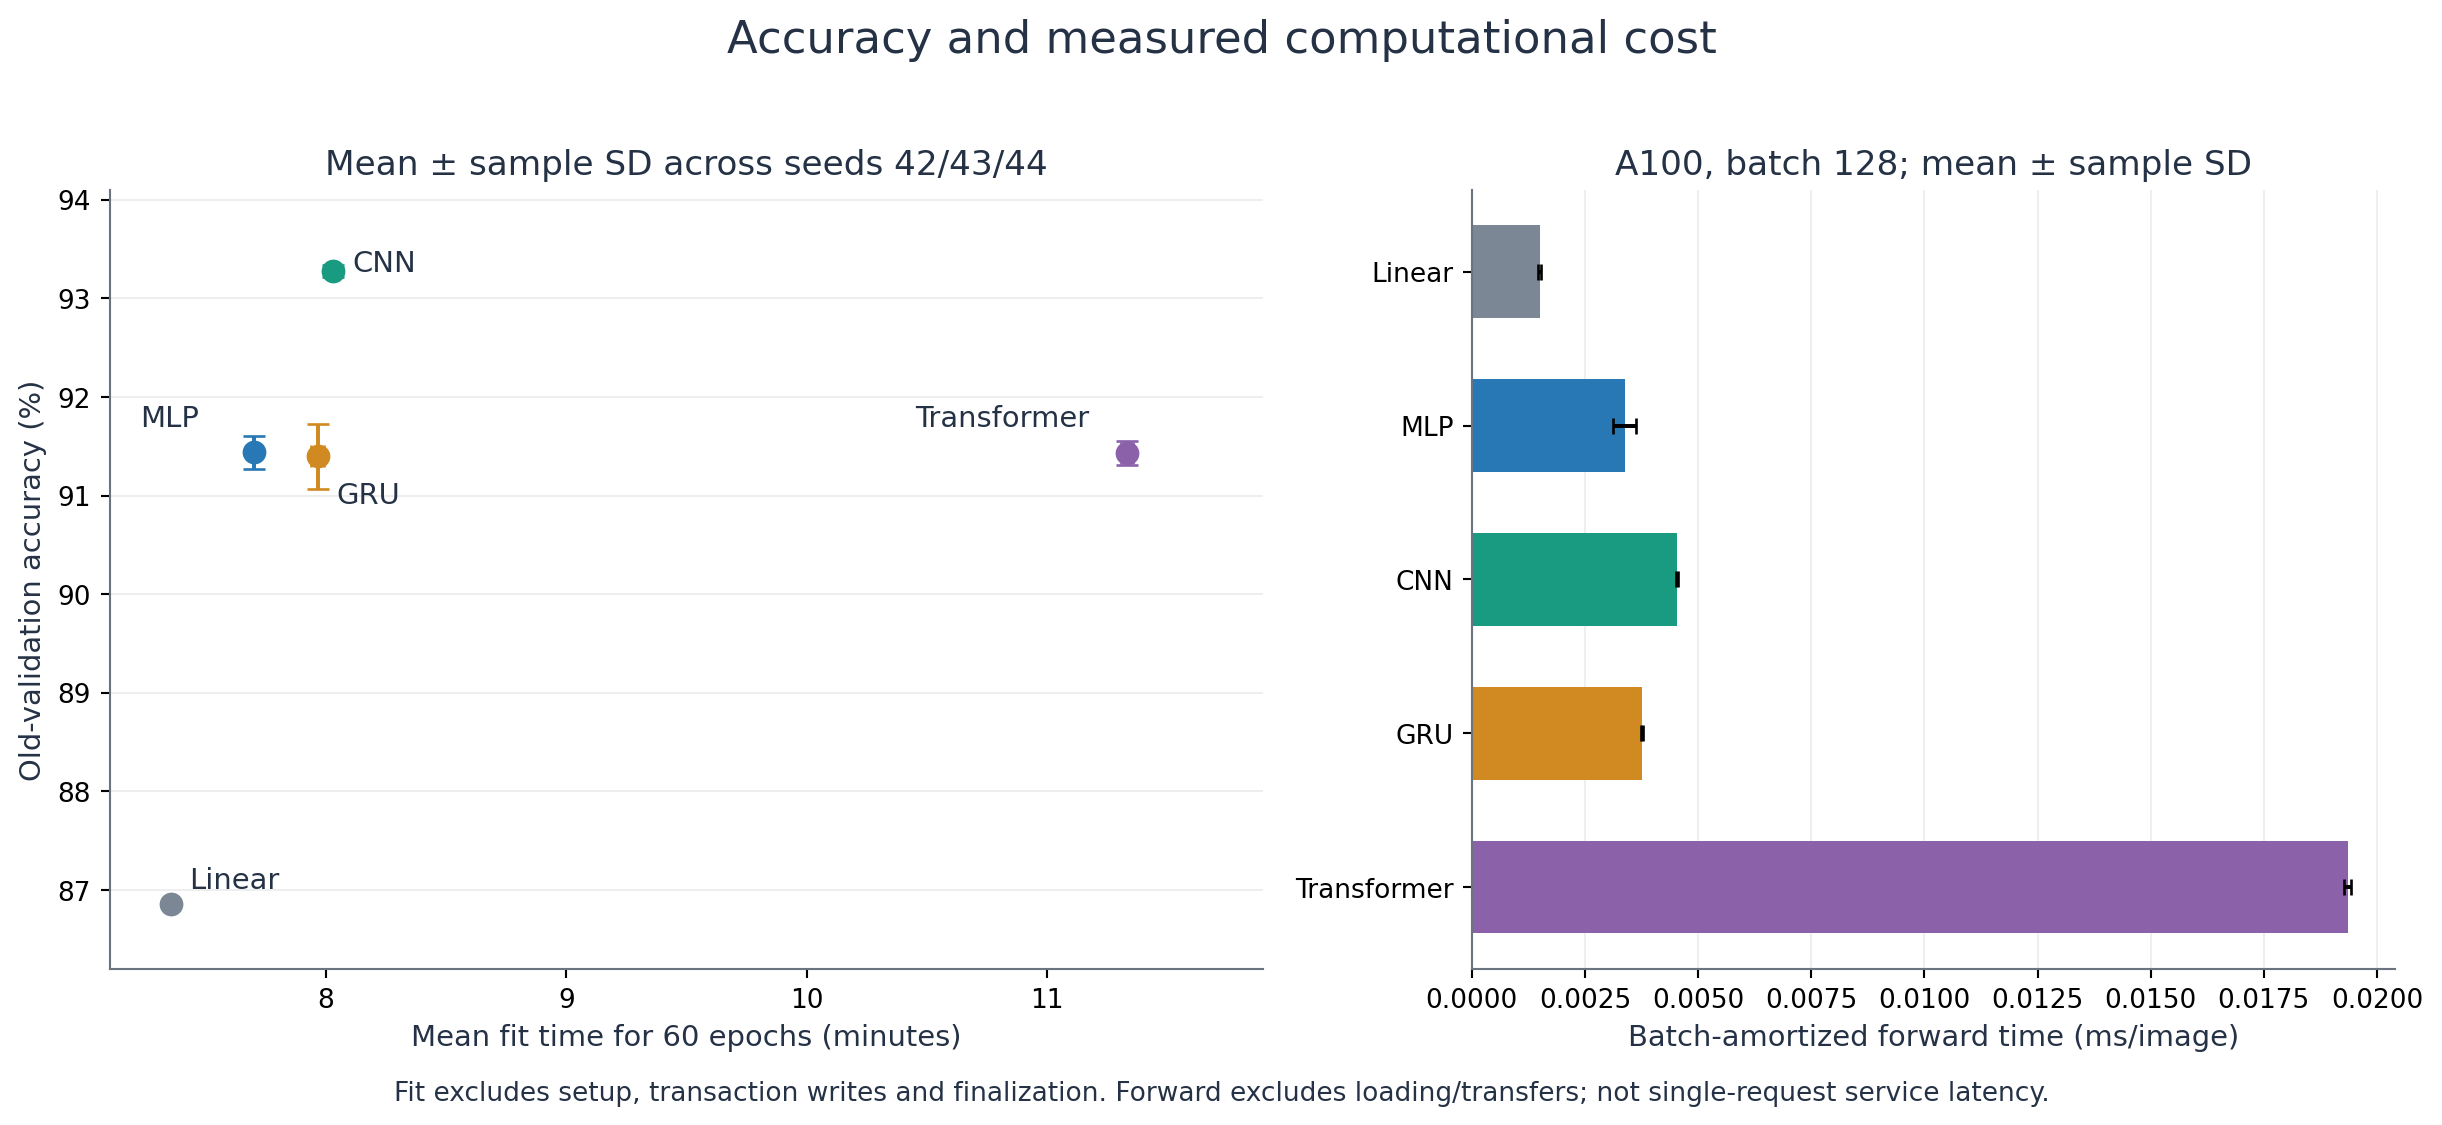
\includegraphics[width=\linewidth]{figures/accuracy_cost.png}
\caption{Final selected recipes: validation accuracy versus mean fit time, and measured batch-amortized forward time. Error bars are sample SD over three seeds. Fit timing and forward timing have different scopes; neither is an energy measurement.}
\label{fig:cost}
\end{figure}
\begin{center}
\small
\begin{tabular}{lrrr}
\toprule
Model & Parameters & Fit seconds & Forward ms/image \\
\midrule
Linear & 7,850 & $441.36 \pm 0.20$ & $0.00150 \pm 0.00003$ \\
MLP & 203,530 & $462.01 \pm 0.47$ & $0.00338 \pm 0.00026$ \\
CNN & 93,962 & $481.90 \pm 0.26$ & $0.00453 \pm 0.00003$ \\
GRU & 61,962 & $477.95 \pm 1.66$ & $0.00375 \pm 0.00002$ \\
Transformer & 274,954 & $679.87 \pm 1.46$ & $0.01935 \pm 0.00007$ \\
\bottomrule
\end{tabular}
\end{center}
\begin{center}
\small
\begin{tabular}{lrrr}
\toprule
Phase & Tasks & Fit minutes & Attempt minutes \\
\midrule
Discovery & 36 & 287.95 & 293.17 \\
Confirmation & 10 & 76.02 & 77.55 \\
Final & 15 & 127.15 & 129.62 \\
\bottomrule
\end{tabular}
\end{center}
The controller's recorded active time is about 8.34 hours. Completed-epoch fit time sums to about 8.19 hours; the sum of task-attempt wall timers is about 8.34 hours. Fit time includes training, validation and in-memory selection, while excluding setup, transaction writes and finalization. The controller clock excludes setup/smoke and may miss an abrupt unrecorded final tail. Their different boundaries account for the differences among these totals.

Forward timing uses A100 inputs already on the device, batch 128, ten warmup batches and 50 measured batches. Dividing batch time by 128 yields amortized milliseconds per image; it is not the latency of one independent service request. The Transformer has the largest parameter count and the highest measured forward cost. CNN combines the highest selected-validation score with 93,962 parameters, fewer than either MLP or Transformer. GRU uses fewer parameters than CNN but has lower mean F1. These are observed operating points, rather than a parameter- or compute-matched architecture experiment.

\clearpage
\section{Discussion and conclusion}
\subsection{What the experiments support}
The original fixed-budget test comparison favors the CNN among the five recorded checkpoints. The final exploratory study also gives CNN the highest validation macro-F1. Its image-specific local structure is consistent with this result, but the experiments do not establish inductive bias as the sole cause: architecture sizes, optimization behavior and training costs differ.

The search finds useful recipe candidates while preserving model size and input processing. The strongest matched-seed inner evidence is the MLP C7 improvement on both seeds. GRU C1 also improves on both, with a smaller margin. CNN's candidate improves on both inner seeds but the fresh-seed gain is much smaller. Linear's effect is small, and Transformer has mixed evidence. Selection and evidence strength therefore differ: the rule determines one recipe, while the paired margins quantify how much support that choice receives.

Checkpoint criterion changes interpretation. Macro-F1 directly targets class-wise classification balance, whereas CE evaluates true-label probabilities. The selected F1 checkpoint can have worse CE than a later or earlier CE-selected alternative. Keeping both artifacts makes that trade-off inspectable. The intended objective determines which checkpoint is appropriate; the recorded study prioritizes class-wise F1.

\subsection{Limits of the claims}
\begin{itemize}
\item The official test was observed before supplementary optimization. Final results are selected, previously seen validation results; no new blind test claim is made.
\item Only one inner split and one fresh confirmation seed are available. Discovery selection and checkpoint selection create additional optimism on those validation sets.
\item Three final training seeds do not measure split variance, population uncertainty or deployment robustness. Small sample SD is not a generalization guarantee.
\item The 61-fit phase did not include fresh final C0 anchors. Its historical CE-selected baseline differences cannot isolate recipe effects. Section~\ref{sec:matched-followup} reports the later matched C0 comparison under a shared checkpoint protocol.
\item The search is intentionally narrow: fixed architecture sizes, fixed optimizer families, no augmentation, no EMA/SWA and no ensemble. Their value remains an open empirical question.
\item Split-ID checks prevent sample-ID overlap; they do not establish absence of near-duplicate content or every possible dataset bias. Runtime is measured with explicit scopes, without energy or production-service measurements.
\end{itemize}

\subsection{Conclusion}
The project provides a reproducible comparison of five deep-learning model families, an original frozen test evaluation and a 61-task exploratory optimization study. The final CNN recipe achieves 93.308\% validation macro-F1 with 0.027 percentage-point seed SD. Across the three research questions, the evidence favors spatial convolution at the measured operating points, supports some recipe changes more consistently than others, and shows that the checkpoint objective changes which epoch is selected. The final 93.308\% Macro-F1 is a selected-validation result. Independent test performance of the optimized checkpoints remains unmeasured. The historical baseline comparison does not isolate HPO effects; the later matched study in Section~\ref{sec:matched-followup} addresses recipe versus checkpoint differences on the same old-validation images.

\clearpage
\clearpage
\part{GarmentLab: RGB transfer learning}
\section{Research questions and data protocol}\label{sec:garmentlab}
GarmentLab extends the from-scratch Fashion-MNIST comparison to six-class classification of selected RGB garment crops with an ImageNet-pretrained encoder. It examines encoder adaptation, controlled regularization and confidence-based review. The different label space and data origin are analyzed separately from the ten-class benchmark.

\subsection{Task, preparation and evaluation units}
Fashionpedia supplies instance-level garment annotations \cite{fashionpedia}. Eligible bounding boxes are mapped to six categories: shirt/blouse, top/T-shirt/sweatshirt, jacket, pants, skirt and dress. Each example is one annotated garment crop; the experiment assumes the region has already been selected. Localization and unrestricted full-image recognition are outside this task.

The prepared subset contains 17,827 crops from 12,419 image IDs. Images are decoded as RGB; bounding-box coordinates use floor for the left/top boundary and ceil for the right/bottom boundary. Crops are letterboxed to $224\times224$ with bilinear resizing and black padding, then normalized with ImageNet channel statistics. Nonidentity EXIF orientation is rejected to preserve the relationship between annotation coordinates and decoded pixels. The metadata eligibility filter accepts license IDs 0, 1 and 6; it records source metadata rather than independently establishing usage rights.

\begin{center}\small
\begin{tabular}{lrrrr}\toprule
Category & Fit & Selection & Calibration & Assessment\\\midrule
Shirt/blouse & 1,284 & 180 & 172 & 19\\
Top/T-shirt/sweatshirt & 3,459 & 461 & 448 & 93\\
Jacket & 1,308 & 183 & 159 & 21\\
Pants & 2,398 & 309 & 295 & 49\\
Skirt & 773 & 107 & 116 & 33\\
Dress & 4,605 & 598 & 645 & 112\\\midrule
Total crops & 13,827 & 1,838 & 1,835 & 327\\
Source groups & 9,610 & 1,274 & 1,302 & 221\\
Duplicate components & 9,339 & 1,265 & 1,243 & 221\\\bottomrule
\end{tabular}\end{center}
Source groups merge records with the same source identity; the number of groups can therefore be smaller than the number of image IDs. Exact decoded-image checks and a perceptual-hash graph at Hamming distance two identify additional duplicate components. Within a cross-role component, the highest-priority role is retained and lower-priority source groups are quarantined, in the order assessment, calibration, selection, then fit. No retained source group spans roles. These checks reduce detectable duplication, but a perceptual-hash component is not a verified garment or person identity.

Fit data update weights. Selection data choose checkpoints and recipes. Calibration data determine confidence scaling and the review policy. The 327 assessment crops originate from the separate validation archive and cover only 221 source groups. They are imbalanced, particularly for shirt/blouse and jacket. The original transfer-learning study used assessment after freezing its choices. Because those outcomes were then inspected, the subsequent tuning study treats the same assessment as \emph{post-test exploratory regression evidence}, rather than a new blind evaluation.

\clearpage
\section{Controlled model comparisons}\label{sec:garmentlab-v2}
\subsection{Encoder adaptation and common training settings}
Both baseline recipes use MobileNetV3-Small \cite{mobilenetv3}, initialized with torchvision's \texttt{IMAGENET1K\_V1} weights and a six-output head. The model has 1,524,006 parameters. Frozen-feature training updates only the final linear layer's 6,150 parameters; fine-tuning updates all parameters. Batch-normalization running statistics retain their ImageNet values in both conditions.

The original comparison uses seeds 314, 2718 and 5772, with 18 epochs per recipe and seed. Paired runs share initial head weights and shuffle/flip random streams. Training uses horizontal flips, AdamW, batch size 128, FP32 arithmetic and gradient clipping at 1. The head learning rate is $10^{-3}$; fine-tuning uses backbone learning rate $3\times10^{-4}$, weight decay $10^{-4}$ and head dropout 0.2. A cosine multiplier decays from 1 toward 0.05. Checkpoints maximize selection Macro-F1, breaking ties by lower clean cross-entropy and then the earliest epoch. The deployment seed is fixed at 314.

\subsection{Regularization search and confirmation}
The follow-up retains the architecture, data roles and training budget, and starts each fit from ImageNet initialization. Eight recipes are declared before their discovery scores are computed. Single-factor probes aid interpretation; combined candidates test a recipe without isolating the contribution of each constituent.

\begin{center}\small
\begin{tabular}{llrr}\toprule
ID & Change from fine-tuning anchor & Discovery F1 & Confirmation F1\\\midrule
C0 & Original anchor & 0.84964 & 0.84082\\
C1 & Backbone LR $10^{-4}$ & 0.82535 & --\\
C2 & Weight decay $10^{-3}$ & 0.84643 & --\\
C3 & Label smoothing 0.05 & 0.84868 & --\\
C4 & Head dropout 0.4 & 0.85388 & 0.84245\\
C5 & Brightness/contrast 0.1 each & 0.84995 & 0.84177\\
C6 & C1 + C2 & 0.82494 & --\\
C7 & C1 + C2 + C3 + C4 + C5 & 0.82641 & --\\\bottomrule
\end{tabular}\end{center}
Discovery seed 101 shortlists C4 and C5. The anchor and both challengers are then fitted with fresh seeds 202 and 303. Their mean selection Macro-F1, excluding discovery scores, selects C4. Its advantage over C0 is 0.00162 F1. The same selection images are reused, so fresh training seeds reduce dependence on one initialization without providing an independent validation sample.

C0 and C4 are subsequently trained with final seeds 314, 2718 and 5772. A preset selection-only guard retains the selected seed-314 model unless its F1 regresses by more than 0.005 relative to C0. The observed difference is $-0.00281$, so C4 remains the selected output. Calibration and assessment do not participate in this decision. Label-smoothed training objectives are recorded separately; selection CE is always unsmoothed and evaluated without augmentation.

The follow-up completes $8+6+6=20$ fits and 360 epochs. Recorded fit timers total 4,593.16 seconds; the controller records 5,380.48 seconds including preparation and finalization. Execution used an NVIDIA A100-SXM4-40GB, Python 3.13.16, PyTorch 2.11.0+cu130, torchvision 0.26.0+cu130, NumPy 2.4.2 and CUDA 13.0. Full candidate values, seeds, source bindings and histories are retained in the experiment manifest.

\clearpage
\section{Classification results and training behavior}
\subsection{Encoder adaptation helps; additional tuning does not establish a gain}
The original fine-tuning recipe improves assessment Macro-F1 over frozen features for every paired seed, with gains 0.1182, 0.0773 and 0.0977. This supports adapting the encoder for the prepared subset. The regularization follow-up yields a different conclusion: C4 slightly improves final selection F1 but has lower mean assessment F1 than C0.

\begin{center}\small
\begin{tabular}{lrrrr}\toprule
& \multicolumn{2}{c}{Selection} & \multicolumn{2}{c}{Assessment}\\
Recipe & Accuracy (\%) & Macro-F1 & Accuracy (\%) & Macro-F1\\\midrule
Frozen features & $80.59\pm0.19$ & $0.76220\pm0.00303$ & $74.41\pm0.18$ & $0.67699\pm0.00553$\\
C0 fine-tuning & $87.21\pm0.24$ & $0.84245\pm0.00597$ & $82.06\pm2.25$ & $0.77472\pm0.01493$\\
C4 dropout 0.4 & $87.25\pm0.36$ & $0.84347\pm0.00383$ & $81.75\pm1.16$ & $0.76638\pm0.02258$\\\bottomrule
\end{tabular}\end{center}
Values are means $\pm$ sample SD over three training seeds on fixed partitions; accuracy SD is in percentage points. The C0 follow-up reproduces the original fine-tuning assessment scores. C4's assessment F1 difference from C0 is $-0.00834$. A paired bootstrap jointly resamples the 221 source/duplicate components across both recipes and their three fixed models, using 2,000 replicates and seed 8601. The descriptive 95\% percentile interval for this mean difference is $[-0.03820,+0.01829]$. It includes zero and supports neither superiority nor equivalence. It describes component sampling on this previously inspected assessment, conditional on the fitted models; it does not account for new training seeds or remove selection bias.

\begin{figure}[H]\centering
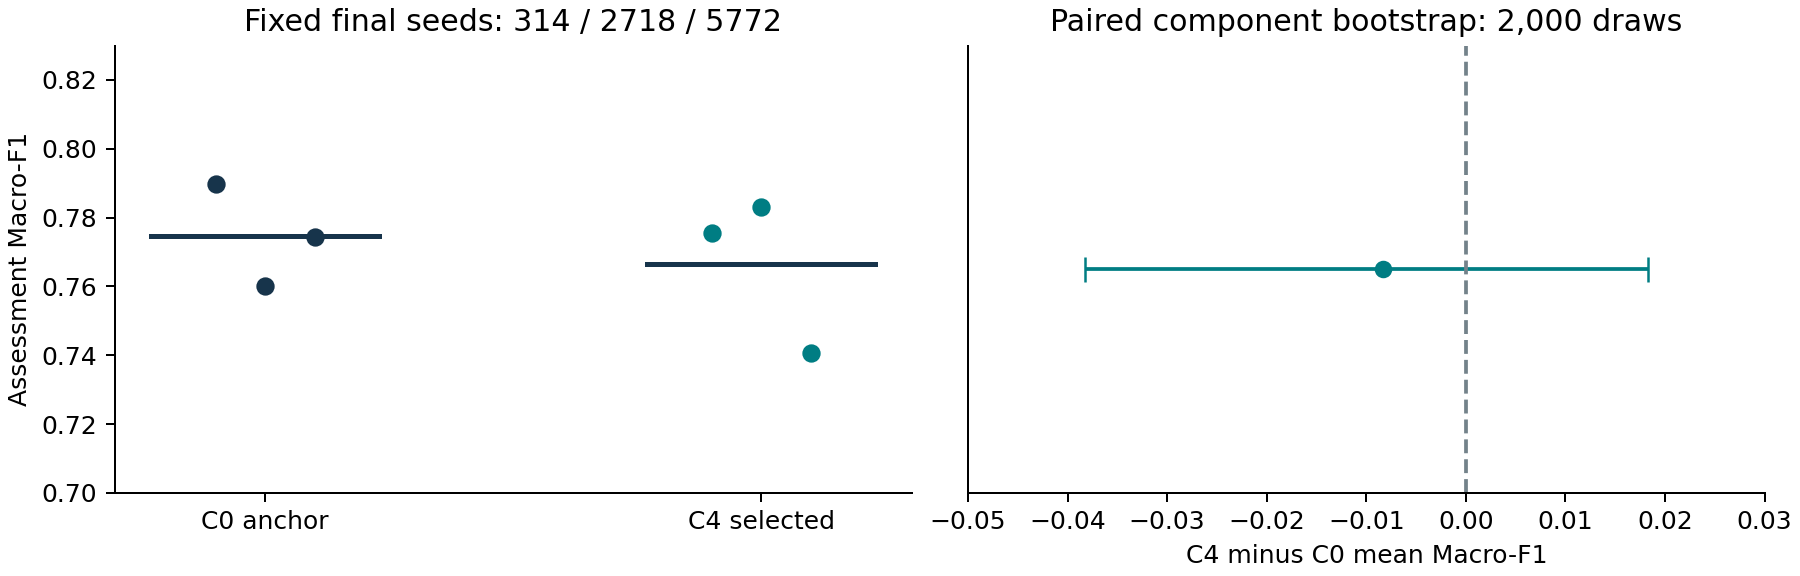
\includegraphics[width=\linewidth]{improve_figures/assessment_comparison.png}
\caption{Final paired assessment results for C0 and C4. Points denote fixed seeds and horizontal marks their means. The interval resamples source/duplicate components jointly rather than treating every crop as independent.}
\label{fig:rgb-paired-assessment}
\end{figure}

\subsection{Overfitting remains visible in loss and accuracy}
For C4 seed 314, training accuracy reaches 99.957\% at epoch 18 while selection accuracy is 87.16\%. Clean selection CE is lowest at epoch 3 (0.42991), then rises to 1.18947 by epoch 18. The F1-selected checkpoint is epoch 17, with selection F1 0.84643 and CE 1.16175. Higher dropout therefore does not eliminate the train--selection gap or excessive raw confidence. Selecting by F1 favors a different objective from minimum CE; each reported row uses metrics from its actual selected checkpoint.

The fixed C4 seed-314 model correctly classifies 269/327 crops (82.26\% accuracy, 0.77553 F1), compared with C0's 274/327 (83.79\%, 0.78989 F1). C4 remains the validation-selected study output, while C0's higher observed assessment score is retained as part of the comparison.

\clearpage
\section{Confidence calibration and selective prediction}
\subsection{Separating probability fitting from threshold selection}
Scalar temperature scaling \cite{temperature} transforms logits $z_k$ into
\[
p_k(x;T)=\frac{\exp(z_k(x)/T)}{\sum_j\exp(z_j(x)/T)},\qquad T\in[0.05,20].
\]
The fitted temperature minimizes calibration NLL. Because $T>0$, scaling preserves class ordering and hence accuracy and Macro-F1. A prediction is accepted automatically when $\max_k p_k(x;T)\ge t$; otherwise it is referred for review. Coverage is the fraction accepted, and accepted accuracy is the correct fraction \emph{within that accepted subset}.

The original C0 procedure fitted temperature and selected an empirical-accuracy threshold on the same calibration partition. The follow-up separates those operations. Joining calibration records by source identity and detected duplicate components produces 1,243 components. A metadata-only split (seed 8401) assigns 621 components, containing 936 crops, to temperature fitting and 622 components, containing 899 crops, to threshold selection. One representative per threshold component is chosen by a seeded hash of annotation identity (seed 8402), before inspecting its logits or label. This avoids counting correlated crops from a component as independent binomial trials and defines an equally weighted representative population.

\subsection{A fixed-grid conditional error bound}
For each threshold in $\{0,0.01,\ldots,1\}$, let $n_t$ and $e_t$ denote accepted representatives and their errors. The one-sided exact Clopper--Pearson upper error limit \cite{exactbinomial} uses significance $0.05/101$. Applying the union bound over the 101 fixed thresholds accounts for selecting a threshold after evaluating the grid. The policy chooses maximum representative coverage among thresholds with $n_t\ge30$ and upper error at most 0.05. If none qualifies, all predictions require review.

For C4, $T=5.345757$ and the selected threshold is $t=0.88$. It accepts 423/622 calibration representatives with six errors, giving 98.58\% empirical accepted accuracy and corrected upper error limit 0.044388. This meets the target \emph{under the binomial assumptions}: a model independent of threshold labels, independent identically distributed representatives, and future data drawn from the same representative population. Historical inspection of calibration, imperfect grouping and deployment shift limit this interpretation. The construction improves data separation and accounts for grid search; it does not supply an unconditional 95\% guarantee for all garment crops or arbitrary photographs.

\begin{figure}[H]\centering
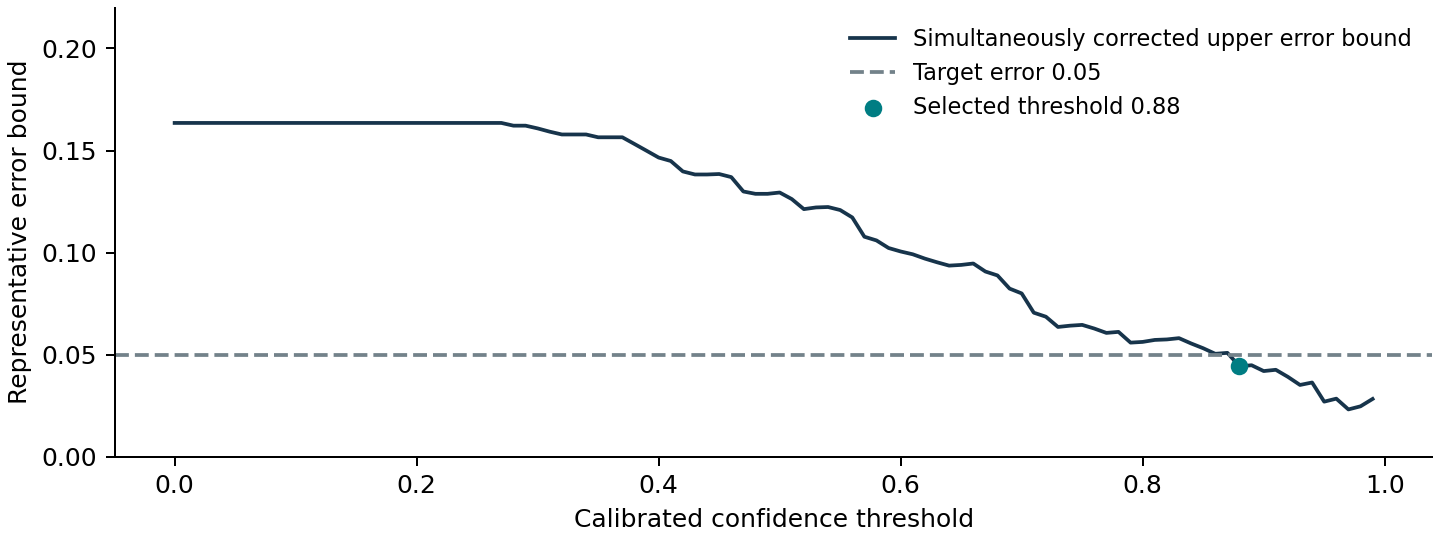
\includegraphics[width=.88\linewidth]{improve_figures/risk_threshold.png}
\caption{Simultaneously corrected upper error limits on the calibration grid, restricted to thresholds accepting at least 30 representatives. The selected threshold 0.88 satisfies the conditional error criterion.}
\label{fig:rgb-risk-bound}
\end{figure}

\clearpage
\section{Reliability, coverage and class-level errors}
\subsection{Calibration changes confidence rather than labels}
Temperatures and thresholds are frozen before assessment inference. Both selected models are overconfident before scaling. NLL and Brier decrease after calibration, while the choice between the calibrated models depends on the metric: C4 has lower ECE but higher NLL than C0.

\begin{center}\small
\begin{tabular}{lrrrr}\toprule
& \multicolumn{2}{c}{C0 seed 314} & \multicolumn{2}{c}{C4 seed 314}\\
Assessment metric & Raw & Calibrated & Raw & Calibrated\\\midrule
Accuracy (\%) & 83.79 & 83.79 & 82.26 & 82.26\\
Macro-F1 & 0.78989 & 0.78989 & 0.77553 & 0.77553\\
NLL & 1.3571 & 0.4843 & 1.5879 & 0.5159\\
Brier score & 0.2899 & 0.2487 & 0.3300 & 0.2618\\
ECE, 15 bins & 0.1339 & 0.0623 & 0.1536 & 0.0499\\\bottomrule
\end{tabular}\end{center}
Brier is the mean sum of squared probability errors across six classes, without division by six. ECE summarizes a particular finite-sample binning and can disagree with proper scoring rules such as NLL and Brier.

\begin{center}\small
\begin{tabular}{lrrrrr}\toprule
Frozen policy & $T$ & Threshold & Correct/accepted & Coverage (\%) & Accepted acc. (\%)\\\midrule
C0, original & 4.922505 & 0.782914 & 211/228 & 69.72 & 92.54\\
C4, disjoint calibration & 5.345757 & 0.88 & 173/182 & 55.66 & 95.05\\\bottomrule
\end{tabular}\end{center}
The C4 policy refers 145 of 327 assessment crops for review. Its accepted-accuracy point estimate is higher than C0's, while coverage falls by 14.07 percentage points and full-sample accuracy is lower. Model and calibration procedure both change between these rows, so the table describes a combined policy outcome rather than isolating a calibration effect. The crop-weighted assessment proportion also differs from the representative-weighted target of the calibration bound.

\subsection{The weakest class is not resolved by tuning}
\begin{center}\small
\begin{tabular}{lrrrr}\toprule
Category & Support & C4 recall (\%) & C0 F1 & C4 F1\\\midrule
Shirt/blouse & 19 & 47.37 & 0.5625 & 0.5806\\
Top/T-shirt/sweatshirt & 93 & 83.87 & 0.8223 & 0.8000\\
Jacket & 21 & 76.19 & 0.8000 & 0.7619\\
Pants & 49 & 87.76 & 0.8980 & 0.8866\\
Skirt & 33 & 66.67 & 0.7667 & 0.7458\\
Dress & 112 & 90.18 & 0.8899 & 0.8783\\\bottomrule
\end{tabular}\end{center}
C4 correctly identifies nine of 19 shirt/blouse crops, with another nine predicted as top/T-shirt/sweatshirt. Dress-to-top confusion contributes nine further errors; six of 33 skirts are classified as dress. These counts identify concrete class boundaries for further analysis. Similar appearance, occlusion, neighboring garments and crop background are plausible contributors, but the experiments do not isolate their causal effects. Small class supports limit the precision of the per-class estimates.

\clearpage
\section{Robustness under fixed perturbations}
The stress suite applies nine predetermined perturbations to already letterboxed assessment arrays. Both checkpoints and their calibration policies remain fixed. Gaussian noise uses standard deviations 0.02, 0.05 and 0.10; blur uses radii 0.5, 1 and 2 pixels; translation uses offsets of 2, 4 and 8 pixels. These synthetic conditions probe specific sensitivities and are not a separate natural-shift dataset.

\begin{center}\small
\begin{tabular}{lrrrr}\toprule
Condition & C0 Macro-F1 & C4 Macro-F1 & C4 coverage (\%) & C4 accepted acc. (\%)\\\midrule
Clean & 0.7899 & 0.7755 & 55.66 & 95.05\\
Noise, $\sigma=0.02$ & 0.7490 & 0.7098 & 51.68 & 94.67\\
Noise, $\sigma=0.05$ & 0.6588 & 0.6711 & 42.81 & 92.86\\
Noise, $\sigma=0.10$ & 0.5512 & 0.6044 & 28.44 & 89.25\\
Blur, radius 0.5 px & 0.7930 & 0.7685 & 55.05 & 94.44\\
Blur, radius 1 px & 0.6952 & 0.7027 & 50.76 & 92.17\\
Blur, radius 2 px & 0.5869 & 0.5941 & 34.86 & 87.72\\
Translation, 2 px & 0.7849 & 0.7279 & 51.38 & 95.24\\
Translation, 4 px & 0.7678 & 0.7418 & 51.68 & 94.67\\
Translation, 8 px & 0.7618 & 0.7825 & 48.62 & 94.34\\\bottomrule
\end{tabular}\end{center}
Strong noise and blur reduce C4 F1 to 0.6044 and 0.5941, decreases of 0.1711 and 0.1814 from its clean result. Although C4 exceeds C0 under these two severe conditions, the relative performance is mixed across the suite. The result is therefore sensitivity to specific perturbations rather than a general robustness advantage for dropout 0.4.

Selective prediction also degrades under these shifts. At the strongest noise and blur settings, accepted accuracy falls to 89.25\% and 87.72\%, despite coverage shrinking to 28.44\% and 34.86\%. Observed accepted accuracy is below 95\% in these conditions; the calibration bound does not certify shifted input populations. Translation results are not monotonic: an eight-pixel shift slightly improves C4 F1 on this finite subset. This can arise from changes in individual crop predictions and does not demonstrate that larger displacement generally helps recognition.

\subsection{What the results support}
The original paired comparison provides consistent evidence that encoder adaptation improves this subset over frozen features. The follow-up does not establish an additional assessment F1 improvement from its selected regularization recipe. Temperature scaling reduces overconfidence, and the stricter selected policy yields higher observed accepted accuracy at lower coverage. Neither regularization nor selective prediction removes the observed class imbalance, overfitting and shift sensitivity.

The distinction between these outcomes matters: a better validation score is not necessarily a better assessment score; a lower ECE is not necessarily a lower NLL; and high accepted accuracy can coexist with lower overall accuracy and substantial human-review workload. Each conclusion concerns its measured population and metric.

\clearpage
\section{Numerical verification and local service behavior}
\subsection{PyTorch execution and ONNX export}
The service processes one selected RGB garment region using the same decoding, crop, letterbox and normalization policy as evaluation. Its release binds weights, label order, preprocessing and calibration parameters. Seven prepared-crop PNG cases exercise the actual image-processing and prediction path; six in-process HTTP checks cover discovery, valid accept/review predictions and invalid-input behavior. Numerical comparisons use a fixed maximum absolute logit tolerance of $10^{-4}$.

\begin{center}\small
\begin{tabular}{p{.43\linewidth}p{.30\linewidth}r}\toprule
Comparison & Recorded cases and batches & Maximum error\\\midrule
C4 PyTorch CPU vs. archived Colab & 327 cases; 1, 3, 64, 128 & $<5.92\times10^{-5}$\\
C4 ONNX, original check & 64 cases; 1, 3, 64 & $9.1970\times10^{-5}$\\
C4 ONNX, expanded check & 327 cases; 1, 3, 64, 128 & $1.3542\times10^{-4}$\\\bottomrule
\end{tabular}\end{center}
The PyTorch comparisons pass, with no label or review-decision differences. The expanded ONNX check fails the fixed numerical tolerance despite matching discrete decisions. Three further CPU exporter/runtime variants also fail that broader criterion. The verified local service consequently uses PyTorch; the ONNX artifact remains experimental. The original 64-case pass and the broader failure are both retained in the evidence.

The CPU checks use Windows, Python 3.12 and PyTorch 2.10, compared with Colab Linux and PyTorch 2.11 for the training return. They test this recorded platform change on the archived cases.

\subsection{End-to-end local HTTP measurement}
A real-server test uses two recorded source JPEG/crop cases, ten warmup requests per supported-concurrency phase and 120 timed predictions each at concurrency one and two. All 240 predictions return HTTP 200. A separate 60.014-second run at concurrency two completes 5,312/5,312 successful predictions: p50 21.70\,ms, p95 31.43\,ms and p99 36.93\,ms, with 88.51 successful predictions/s. Client timing includes multipart construction, loopback transfer, decoding, preprocessing, forward execution and response serialization; source-file reads precede timing.

A 24-request overload probe at concurrency eight produces nine successful predictions and 15 expected busy responses, with no unexpected failures. Invalid-input tests return the recorded 400, 400, 415 and 413 statuses. Successful-prediction throughput is kept separate from attempted requests and overload responses. This short, repeated-input loopback experiment characterizes the local service, not hosted availability or production capacity.

\subsection{Reproducibility and extension conclusion}
The record retains data roles, candidate values, 20 histories, checkpoint decisions, predictions and source bindings. Its audit verifies 273 payload hashes and reconstructs classification metrics, temperature, all 101 threshold bounds and the component bootstrap. A clean isolated environment passes 261 software tests with two condition-dependent skips.

Paired evidence supports encoder adaptation on this subset. Subsequent regularization does not establish a further F1 gain, while calibration trades coverage for higher observed accepted accuracy. Class errors, shift sensitivity and ONNX numerical failure remain. Section~\ref{sec:prospective-followup} reports a later locked cohort from previously unused source groups. Broader service and external-population testing remain necessary for operational conclusions.

\clearpage
\clearpage
\part{Matched confirmation and prospective audit}
\section{Recipe effects under matched training}\label{sec:matched-confirmation}\label{sec:matched-followup}
The follow-up tests two weaknesses in the earlier evidence: the absence of freshly fitted C0 anchors under the final training engine, and the limited independent RGB assessment. Its protocol fixes the comparisons before the new runs. The grayscale and RGB experiments remain separate tasks; the RGB cohort does not provide a new test for Fashion-MNIST.

For each Fashion-MNIST family, the original C0 recipe and the frozen OPT3-selected recipe are trained for 60 epochs with fresh seeds 1009, 2027 and 3037. Paired arms share the exact 54,000/6,000 split, engine, architecture dimensions, initialization policy and loader seed. Recipe order alternates by seed. Each trajectory supplies minimum-CE, maximum-F1 and fixed-epoch-60 checkpoints: 30 fits yield 90 checkpoint cells, not 90 independent fits.

The prespecified primary contrast is selected recipe minus C0 for the CNN at epoch 60. Other families, adaptive checkpoint policies and their interaction are secondary descriptive comparisons. The design separates a recipe bundle from checkpoint selection, rather than isolating individual learning-rate, regularization or scheduling effects.

\begin{center}\small
\setlength{\tabcolsep}{4pt}
\begin{tabular}{lrrrr}\toprule
Family & C0, epoch 60 & Selected, epoch 60 & Paired difference & Positive pairs\\\midrule
Linear & $0.86280\pm0.00211$ & $0.86618\pm0.00094$ & $+0.00338\pm0.00143$ & 3/3\\
MLP & $0.90218\pm0.00236$ & $0.91109\pm0.00206$ & $+0.00891\pm0.00115$ & 3/3\\
CNN & $0.92823\pm0.00087$ & $0.92914\pm0.00273$ & $+0.00091\pm0.00351$ & 1/3\\
GRU & $0.90293\pm0.00298$ & $0.90615\pm0.00278$ & $+0.00322\pm0.00374$ & 2/3\\
Transformer & $0.90228\pm0.00297$ & $0.91174\pm0.00087$ & $+0.00946\pm0.00247$ & 3/3\\\bottomrule
\end{tabular}\end{center}
All scores are Macro-F1, with mean $\pm$ sample SD over three seeds. Difference SD is calculated from paired seed differences. These are descriptive SDs on a fixed, previously inspected validation split, not population confidence intervals.

\subsection{The primary CNN gain is small and inconsistent}
The primary mean difference is $+0.000912$ F1, or $0.0912$ F1 percentage points. Its paired differences are $+0.004894$, $-0.001738$ and $-0.000419$ for seeds 1009, 2027 and 3037. Only one pair favors C5, and the paired SD of 0.003511 exceeds the mean effect. This does not establish a stable recipe improvement. C5 also has greater between-seed variability at epoch 60 than C0 in this run.

MLP and Transformer have larger positive final-epoch differences in all three pairs. These secondary outcomes support better late-trajectory behavior for their selected recipes under the declared protocol. They remain conditional on configurations chosen during earlier development and on a reused validation sample. Fresh training seeds reduce dependence on one initialization; they do not create fresh evaluation images.

\clearpage
\section{Checkpoint dependence and objective trade-offs}
\begin{center}\small
\setlength{\tabcolsep}{5pt}
\begin{tabular}{lrrrrrr}\toprule
& \multicolumn{2}{c}{Minimum CE} & \multicolumn{2}{c}{Maximum F1} & \multicolumn{2}{c}{Epoch 60}\\
Family & C0 & Selected & C0 & Selected & C0 & Selected\\\midrule
Linear & 0.86504 & 0.86481 & 0.86830 & 0.86806 & 0.86280 & 0.86618\\
MLP & 0.90200 & 0.91021 & 0.90866 & 0.91360 & 0.90218 & 0.91109\\
CNN & 0.92877 & 0.92940 & 0.92991 & 0.93126 & 0.92823 & 0.92914\\
GRU & 0.90962 & 0.90959 & 0.91294 & 0.91278 & 0.90293 & 0.90615\\
Transformer & 0.90630 & 0.90592 & 0.91022 & 0.91326 & 0.90228 & 0.91174\\\bottomrule
\end{tabular}\end{center}
Entries are mean validation Macro-F1 over the same three seeds. All checkpoints in a row/arm derive from its shared 60-epoch trajectories.

The CNN recipe difference is $+0.000635$ at the CE-selected checkpoint and $+0.001351$ at the F1-selected checkpoint. The latter favors C5 in all three pairs, but it is a secondary adaptive comparison and does not override the weak primary result. The recipe-by-selector interaction,
\[
  (\mathrm{selected}_{F1}-\mathrm{C0}_{F1})
  -(\mathrm{selected}_{CE}-\mathrm{C0}_{CE}),
\]
is $+0.000716\pm0.001736$ for the CNN. Its variation across three pairs does not support a population interaction claim.

For Linear, cosine scheduling improves epoch-60 F1 by 0.00338 while recipe differences at CE/F1-selected checkpoints are approximately zero ($-0.00023/-0.00024$). GRU shows the same pattern: $+0.00322$ at epoch 60, but $-0.00003/-0.00016$ after CE/F1 selection. Transformer has differences $+0.00946$, $-0.00038$ and $+0.00304$ at final, CE and F1 checkpoints respectively. Thus an improvement at the end of training is not interchangeable with superiority of a validation-selected checkpoint.

\subsection{Higher selected validation F1 does not establish generalization}
Maximum-F1 selection explicitly maximizes the same validation score reported here. Its score being at least as high as that of the CE-selected checkpoint on those images is expected by construction. The within-trajectory comparison describes the choice of objective; it cannot independently demonstrate better generalization.

The losses illustrate the distinction. For MLP C0, mean validation CE is 0.27457 at the CE checkpoint, 0.32177 at the F1 checkpoint and 0.40553 at epoch 60. A checkpoint with higher F1 can have worse probability loss. The final-epoch primary endpoint avoids within-trajectory validation selection, but it still uses images repeatedly inspected during project development. No official-test evaluation is performed in this follow-up.

\subsection{Completion and numerical portability}
All 30 trajectories finish 60 epochs and 25,320 optimizer updates. The A100 controller records 15,335.76 active seconds (4.260 hours), excluding setup and the initial software smoke test. The environment is PyTorch 2.11.0+cu130, torchvision 0.26.0+cu130, NumPy 2.4.2, scikit-learn 1.8.0 and Python 3.13 on an NVIDIA A100-SXM4-40GB.

Independent reconstruction verifies all 540,000 prediction rows, 90 cells, 1,800 history rows, validation IDs and checkpoint epochs (maximum metric difference $2.23\times10^{-16}$). NLL checks aggregate the saved per-image values. Read-only CPU/PyTorch 2.10 replay strictly loads all 90 checkpoints, recording 11 label differences across 540,000 cell-image predictions and maximum cell mean-NLL difference $1.55\times10^{-5}$. Tables retain the original A100 values; exact cross-runtime identity is not claimed. The primary CNN conclusion is unchanged.

\clearpage
\section{A prospectively fixed RGB cohort}\label{sec:prospective-rgb}\label{sec:prospective-followup}
\subsection{Cohort construction and fixed model identities}
The new audit uses photographs from Fashionpedia training license IDs 3/5, excluded by the earlier 0/1/6 filter. Six previously fitted C0/C4 checkpoints, seeds 314/2718/5772, preprocessing, the C4 seed-314 review policy and analysis are frozen before cohort preparation. There is no new RGB fitting, calibration or threshold selection.

Source-URL groups are ranked by SHA256 with seed 20261029. The first 2,000 groups are committed before target-category filtering, without replacement after exclusions. Recorded image IDs, source URLs, previews and quarantines are excluded. Transitive exact-pixel/perceptual-hash components touching historical images are removed. These controls reduce detectable overlap but cannot guarantee separation of every person, outfit or undetected near-duplicate.

The final cohort contains 2,766 annotated crops in 1,826 source/duplicate components. Inference was completed locally on CPU before the Colab confirmation run. Colab reuses the frozen audit evidence byte for byte; this is not a second independent RGB evaluation. The cohort remains a project-unused, same-source license-shift audit, rather than an external or IID benchmark. Unrecorded prior viewing and pretrained-model exposure cannot be excluded. Photographs and prepared crops are not redistributed.

\begin{center}\small
\begin{tabular}{lrrrr}\toprule
Category & Crops & Components & C0 mean F1 & C4 mean F1\\\midrule
Shirt/blouse & 182 & 175 & 0.5633 & 0.5659\\
Top/T-shirt/sweatshirt & 856 & 811 & 0.8123 & 0.8208\\
Jacket & 300 & 279 & 0.7211 & 0.7395\\
Pants & 476 & 461 & 0.9091 & 0.9185\\
Skirt & 257 & 253 & 0.7840 & 0.7856\\
Dress & 695 & 684 & 0.8572 & 0.8589\\\bottomrule
\end{tabular}\end{center}
Components can contain several categories, so class-level component counts do not sum to the cohort total. Shirt/blouse remains the weakest category despite greater support than the original assessment; aggregate accuracy does not describe uniform class performance.

\subsection{A favorable point estimate with unresolved uncertainty}
\begin{center}\small
\setlength{\tabcolsep}{4pt}
\begin{tabular}{lrrrr}\toprule
Cohort & C0 F1 & C4 F1 & Difference & Paired 95\% interval\\\midrule
Earlier assessment (327) & 0.77472 & 0.76638 & $-0.00834$ & $[-0.03820,+0.01829]$\\
Project-unused cohort (2,766) & 0.77449 & 0.78154 & $+0.00705$ & $[-0.00036,+0.01512]$\\\bottomrule
\end{tabular}\end{center}
The prespecified RGB endpoint is C4 minus C0 mean Macro-F1 over three paired fixed models. On the new cohort the mean difference is $+0.007046$, or 0.7046 F1 percentage points. A 2,000-replicate paired percentile bootstrap resamples the 1,826 source/duplicate components jointly, with seed 20261030. Its interval includes zero. It describes component-sampling uncertainty conditional on these six models, without seed-population, external-data or deployment guarantees. It establishes neither a positive effect nor equivalence. The opposite direction on the earlier assessment is retained.

\clearpage
\section{Frozen review policy by garment class}\label{sec:policy-by-class}
\subsection{Global result and true-class behavior}
This diagnostic concerns the single, preselected C4 seed-314 model. It is separate from the preceding three-seed mean-F1 comparison. For logits $z_i$, the policy computes $\pi_i=\operatorname{softmax}(z_i/T)$ with the frozen temperature $T=5.345757234366385$, predicts $\hat Y_i=\arg\max_k\pi_{ik}$, and accepts when
\[
 A_i=\mathbf{1}\!\left[\max_k\pi_{ik}\geq0.88\right].
\]
The remaining crops are referred for review. Positive temperature scaling leaves the predicted class unchanged. No weights, temperature or threshold are fitted or changed in this post-hoc analysis of stored logits and labels.

The policy accepts 1,506/2,766 crops (54.45\% coverage), of which 1,445 are correct (95.95\% accepted accuracy). It refers 1,260 crops and retains 61 errors among accepted predictions. Full-cohort accuracy remains 82.1041\% and Macro-F1 0.783914. These different denominators describe different aspects of the same fixed model.

For a true class $Y=c$, coverage measures its accepted fraction, and accepted accuracy measures correctness within that fraction:
\[
 \widehat C^Y_c=\frac{\sum_i A_i\mathbf{1}(Y_i=c)}{\sum_i\mathbf{1}(Y_i=c)},
 \qquad
 \widehat a^{Y,A}_c=\frac{\sum_i A_i\mathbf{1}(Y_i=\hat Y_i=c)}{\sum_i A_i\mathbf{1}(Y_i=c)}.
\]
\begin{center}\small
\setlength{\tabcolsep}{4pt}
\begin{tabular}{lrrrrr}\toprule
True category & Accepted/total & Correct/accepted & Review & \shortstack{Coverage\\(\%)} & \shortstack{Accepted\\accuracy (\%)}\\\midrule
Shirt/blouse & 33/182 & 22/33 & 149 & 18.13 & 66.67\\
\shortstack[l]{Top/T-shirt/\\sweatshirt} & 431/856 & 406/431 & 425 & 50.35 & 94.20\\
Jacket & 82/300 & 76/82 & 218 & 27.33 & 92.68\\
Pants & 361/476 & 360/361 & 115 & 75.84 & 99.72\\
Skirt & 106/257 & 100/106 & 151 & 41.25 & 94.34\\
Dress & 493/695 & 481/493 & 202 & 70.94 & 97.57\\\midrule
Total & 1,506/2,766 & 1,445/1,506 & 1,260 & 54.45 & 95.95\\\bottomrule
\end{tabular}\end{center}
The global result masks substantial class variation. Of 182 true shirt/blouse crops, 149 are referred; 11 of the 33 accepted crops are still misclassified. Pants have much higher coverage and only one error among 361 accepted crops. Shirt/blouse contributes 2.19\% of the accepted set but 18.03\% of its errors. A high pooled accepted accuracy therefore does not establish reliable handling of every garment category.

This grouping evaluates labeled audit data. The true class is unavailable when a new crop arrives, so these rows cannot directly specify an online class-dependent acceptance rule. The small accepted shirt/blouse count also limits precision of its rate estimate. The counts are descriptive outcomes on this cohort, not per-class accuracy guarantees.

\clearpage
\subsection{Predicted outputs and review workload}
Grouping by predicted class answers a different question: how reliable is an accepted output labeled $c$? Predicted-class coverage estimates $\Pr(A=1\mid\hat Y=c)$, while accepted precision estimates $\Pr(Y=c\mid A=1,\hat Y=c)$. The denominators now include all predictions of $c$, rather than all crops whose true class is $c$. Predicted labels are observable online; measuring their precision still requires ground-truth audit labels.

\begin{center}\small
\setlength{\tabcolsep}{4pt}
\begin{tabular}{lrrrrr}\toprule
Predicted output & \shortstack{Accepted/\\predictions} & Correct/accepted & Review & \shortstack{Coverage\\(\%)} & \shortstack{Accepted\\precision (\%)}\\\midrule
Shirt/blouse & 24/183 & 22/24 & 159 & 13.11 & 91.67\\
\shortstack[l]{Top/T-shirt/\\sweatshirt} & 428/856 & 406/428 & 428 & 50.00 & 94.86\\
Jacket & 88/284 & 76/88 & 196 & 30.99 & 86.36\\
Pants & 362/484 & 360/362 & 122 & 74.79 & 99.45\\
Skirt & 101/243 & 100/101 & 142 & 41.56 & 99.01\\
Dress & 503/716 & 481/503 & 213 & 70.25 & 95.63\\\midrule
Total & 1,506/2,766 & 1,445/1,506 & 1,260 & 54.45 & 95.95\\\bottomrule
\end{tabular}\end{center}
Accepted jacket outputs have the lowest observed precision, 76/88 = 86.36\%. Accepted outputs labeled shirt/blouse have precision 22/24 = 91.67\%; this is not the 22/33 true-class accepted accuracy in the preceding table. The two rates condition on different events and must not be interchanged.

The accepted confusion counts explain why this distinction matters. The 11 accepted errors on true shirt/blouse crops are labeled jacket (five), top/T-shirt/sweatshirt (four) or dress (two). A change applied only to outputs predicted as shirt/blouse would not directly address those 11 cases. Of the 12 false accepted jacket outputs, six are true tops, five are true shirts/blouses and one is a true dress. These are observed confusion patterns, without a claim about their visual cause.

Across all classes, the model makes 495 full-cohort errors. The policy refers 434 of them for review (87.68\%) and accepts the other 61. The review stream also contains 826 predictions that were already correct. Referral therefore trades automatic coverage for review workload; it does not measure how accurately a human would resolve those crops. Human-review outcomes, processing time and costs are unmeasured.

\subsection{Scope of the policy conclusion}
This class breakdown was added after cohort outcomes were inspected. Crops share source/duplicate components, and small accepted subsets warrant caution. The earlier representative-level calibration bound was neither a per-class certificate nor a guarantee for this license-shifted population. Neither table establishes that every class meets 95\% accepted accuracy. Conditioning on the true label also differs from conditioning on confidence, so the shirt/blouse row is not a direct test of probability calibration.

A class-aware policy would require its own suitable calibration evidence and a prespecified evaluation on another untouched cohort. No such policy is selected here, and the threshold remains 0.88. The matched recipe and grouped RGB comparisons retain their earlier conclusions. This diagnostic qualifies the interpretation of selective operation without replacing either primary endpoint or the recorded local-serving and ONNX limitations.

\clearpage
\section{Paired diagnostic plots}
\begin{figure}[H]
\centering
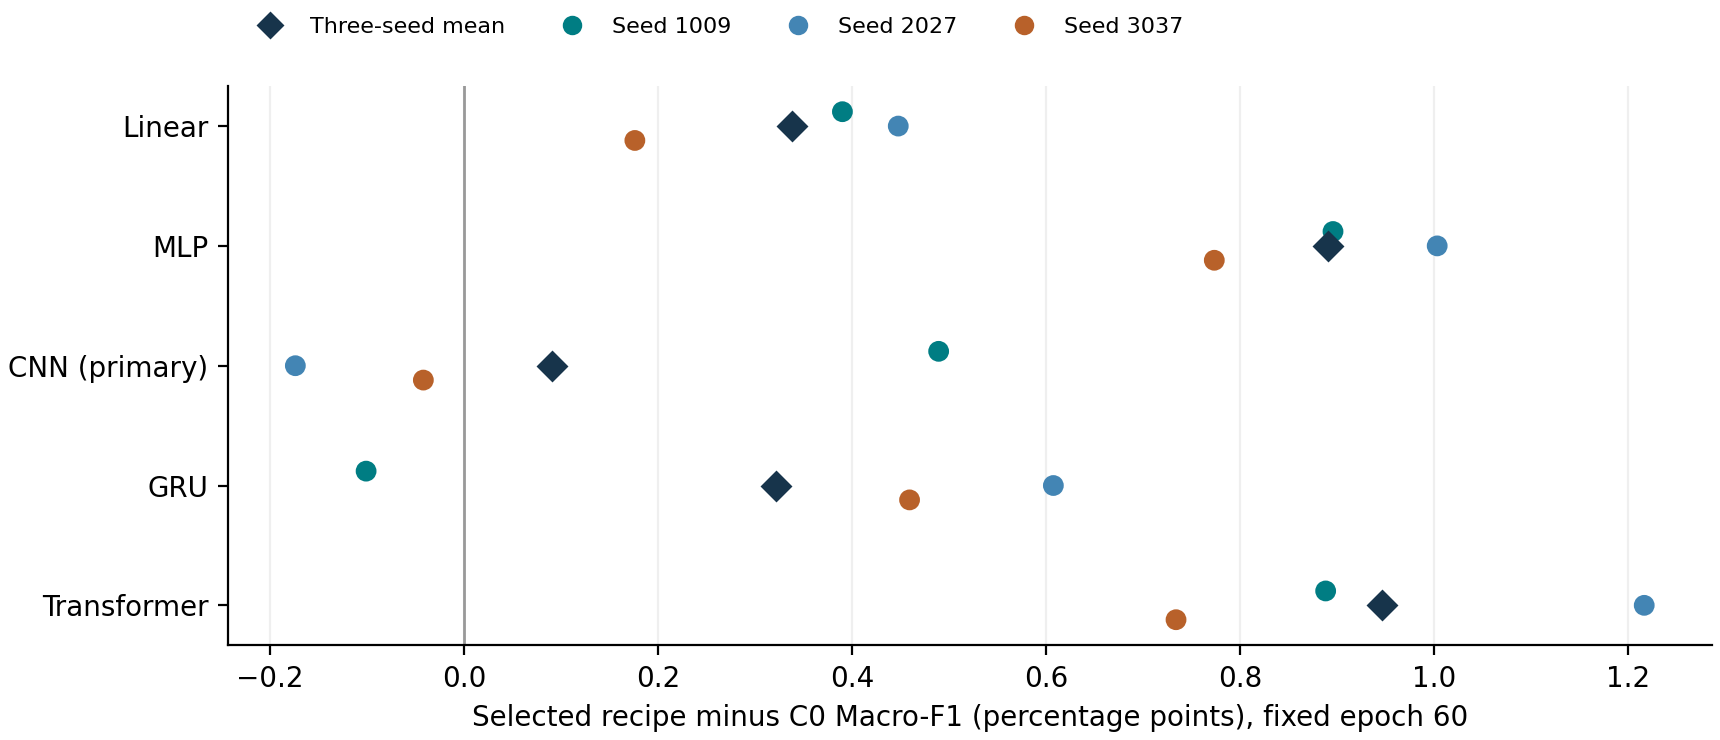
\includegraphics[width=\linewidth]{figures/matched_epoch60_deltas.png}
\caption{Fixed-epoch-60 recipe differences on the old validation partition. Each circle is one paired training seed; diamonds are three-seed means. The prespecified primary family is CNN. The displayed dispersion concerns training seeds on one fixed split, without a new image-population confidence claim.}
\end{figure}
\begin{figure}[H]
\centering
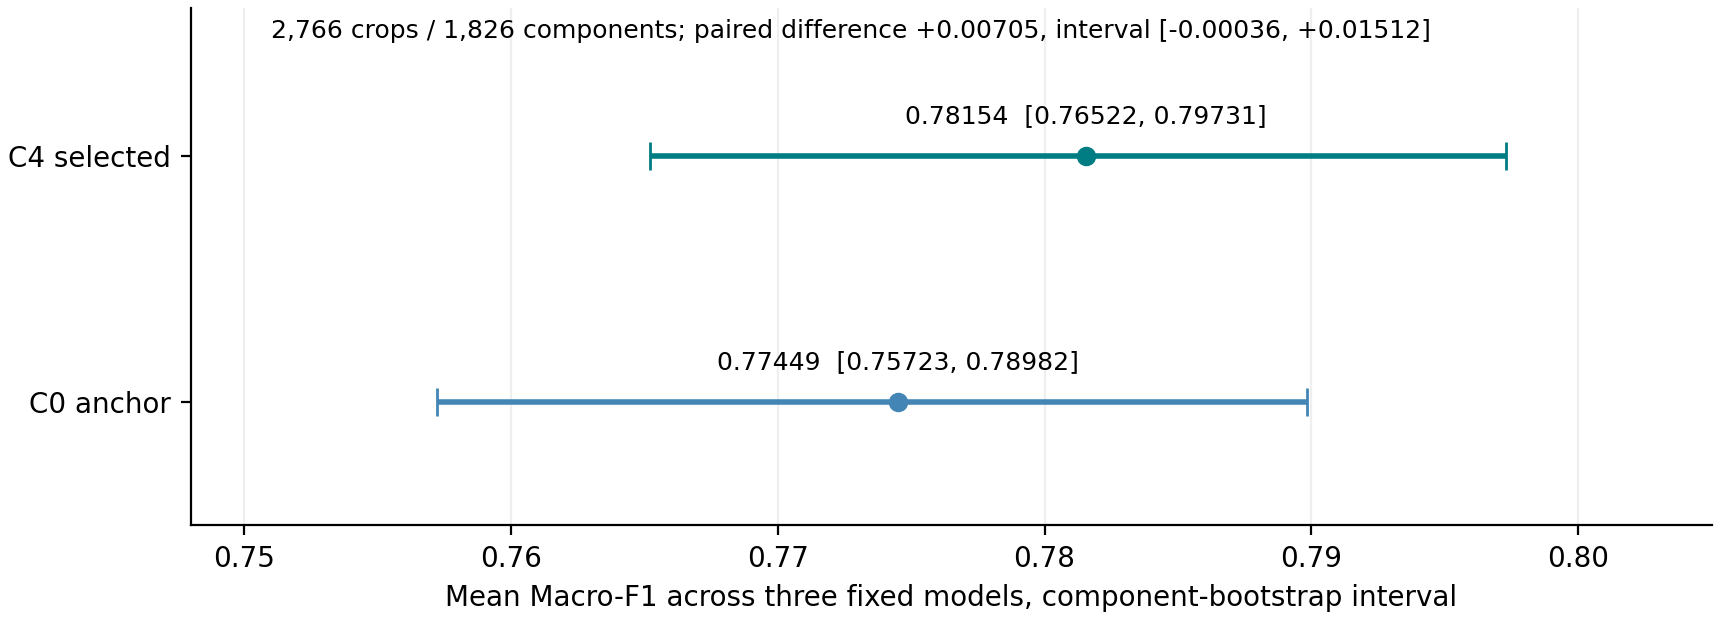
\includegraphics[width=\linewidth]{figures/prospective_rgb_intervals.png}
\caption{Mean Macro-F1 on the project-unused RGB cohort. Marginal component-bootstrap intervals describe the six fixed fitted models. The joint paired difference interval, shown in the plot, is the relevant recipe contrast and includes zero. Overlap of marginal intervals is not used as a significance test.}
\end{figure}

\clearpage
\appendix
\section{OPT3 per-seed results}\label{app:seeds}
Every row is a separate completed 60-epoch final fit on 54,000 training images, selected on the same 6,000-image old-validation partition. The epoch column is the F1-selected checkpoint; it is not the number of epochs executed.

\begin{center}
\small
\begin{tabular}{lcrrrrrr}
\toprule
Model & ID & Seed & Epoch & Acc.(\%) & F1(\%) & CE & Fit(s) \\
\midrule
Linear & C1 & 42 & 40 & 86.850 & 86.876 & 0.38007 & 441.25 \\
Linear & C1 & 43 & 41 & 86.850 & 86.828 & 0.37832 & 441.60 \\
Linear & C1 & 44 & 35 & 86.867 & 86.850 & 0.37865 & 441.25 \\
MLP & C7 & 42 & 56 & 91.500 & 91.501 & 0.26230 & 462.55 \\
MLP & C7 & 43 & 47 & 91.250 & 91.276 & 0.26441 & 461.76 \\
MLP & C7 & 44 & 58 & 91.567 & 91.568 & 0.26235 & 461.72 \\
CNN & C5 & 42 & 44 & 93.283 & 93.295 & 0.19159 & 481.63 \\
CNN & C5 & 43 & 60 & 93.217 & 93.290 & 0.19119 & 481.90 \\
CNN & C5 & 44 & 55 & 93.333 & 93.339 & 0.19174 & 482.16 \\
GRU & C1 & 42 & 37 & 91.350 & 91.324 & 0.27978 & 476.13 \\
GRU & C1 & 43 & 28 & 91.750 & 91.762 & 0.25923 & 478.33 \\
GRU & C1 & 44 & 34 & 91.100 & 91.014 & 0.28524 & 479.39 \\
Transformer & C1 & 42 & 58 & 91.567 & 91.541 & 0.32483 & 681.46 \\
Transformer & C1 & 43 & 48 & 91.400 & 91.395 & 0.31269 & 679.56 \\
Transformer & C1 & 44 & 41 & 91.333 & 91.358 & 0.29000 & 678.59 \\
\bottomrule
\end{tabular}
\end{center}
\subsection{Checkpoint contrast for CNN C5, seed 42}

\begin{center}
\small
\begin{tabular}{lrrrr}
\toprule
Selection & Epoch & Accuracy(\%) & Macro-F1(\%) & CE \\
\midrule
Maximum F1 & 44 & 93.283 & 93.295 & 0.191585 \\
Minimum CE & 51 & 93.267 & 93.282 & 0.187897 \\
Last epoch & 60 & 92.700 & 92.635 & 0.206214 \\
\bottomrule
\end{tabular}
\end{center}
The selected-epoch examples in the main text use saved predictions from the F1 checkpoint. The loss column can be checked by averaging the supplied per-image negative log-likelihood values. Accuracy and macro-F1 are independently reconstructed from class counts. Without logits, the artifact review validates NLL aggregation rather than independently recomputing softmax probabilities.

\clearpage
\section{Realized candidate recipes}\label{app:recipes}
The following 36 rows are the actual discovery manifest. LR values are rounded here for readability; machine-readable configurations retain full precision. ``Drop'' denotes the effective hidden/head/encoder dropout appropriate to that family. The architecture widths and optimizer families are held fixed. C0 is the anchor, C1 the schedule probe; nonlinear C2 is the targeted probe. The remaining rows are sampled candidates from the declared search space.

\begin{center}\footnotesize
\begin{longtable}{llrrlllr}
\toprule
Family & ID & LR & Decay & Drop & Schedule & Init & Discovery F1(\%)\\
\midrule\endfirsthead
\toprule
Family & ID & LR & Decay & Drop & Schedule & Init & Discovery F1(\%)\\
\midrule\endhead

Linear & C0 & $1.000\!\times\!10^{-3}$ & $0$ & 0 & const. & legacy & 85.655 \\
Linear & C1 & $1.000\!\times\!10^{-3}$ & $0$ & 0 & cosine & legacy & 85.657 \\
Linear & C2 & $7.136\!\times\!10^{-4}$ & $1.000\!\times\!10^{-4}$ & 0 & const. & legacy & 85.516 \\
Linear & C3 & $2.740\!\times\!10^{-3}$ & $1.000\!\times\!10^{-3}$ & 0 & cosine & legacy & 85.398 \\
MLP & C0 & $1.000\!\times\!10^{-3}$ & $0$ & 0 & const. & legacy & 89.897 \\
MLP & C1 & $1.000\!\times\!10^{-3}$ & $0$ & 0 & cosine & legacy & 90.296 \\
MLP & C2 & $1.000\!\times\!10^{-3}$ & $0$ & 0.2 & const. & legacy & 89.981 \\
MLP & C3 & $4.168\!\times\!10^{-4}$ & $1.000\!\times\!10^{-5}$ & 0.3 & const. & legacy & 90.114 \\
MLP & C4 & $9.448\!\times\!10^{-4}$ & $1.000\!\times\!10^{-5}$ & 0.3 & cosine & legacy & 90.352 \\
MLP & C5 & $1.599\!\times\!10^{-3}$ & $0$ & 0 & cosine & legacy & 90.071 \\
MLP & C6 & $1.289\!\times\!10^{-3}$ & $1.000\!\times\!10^{-5}$ & 0.3 & const. & legacy & 89.853 \\
MLP & C7 & $1.010\!\times\!10^{-3}$ & $1.000\!\times\!10^{-5}$ & 0.2 & cosine & legacy & 90.411 \\
CNN & C0 & $1.000\!\times\!10^{-3}$ & $1.000\!\times\!10^{-4}$ & 0.2 & const. & legacy & 92.095 \\
CNN & C1 & $1.000\!\times\!10^{-3}$ & $1.000\!\times\!10^{-4}$ & 0.2 & cosine & legacy & 91.709 \\
CNN & C2 & $1.000\!\times\!10^{-3}$ & $1.000\!\times\!10^{-3}$ & 0.2 & const. & legacy & 92.219 \\
CNN & C3 & $1.521\!\times\!10^{-3}$ & $1.000\!\times\!10^{-5}$ & 0.1 & cosine & legacy & 92.559 \\
CNN & C4 & $1.008\!\times\!10^{-3}$ & $1.000\!\times\!10^{-3}$ & 0.2 & cosine & legacy & 91.656 \\
CNN & C5 & $1.438\!\times\!10^{-3}$ & $1.000\!\times\!10^{-4}$ & 0.3 & const. & legacy & 92.662 \\
CNN & C6 & $8.522\!\times\!10^{-4}$ & $1.000\!\times\!10^{-5}$ & 0.1 & cosine & legacy & 91.084 \\
CNN & C7 & $7.314\!\times\!10^{-4}$ & $1.000\!\times\!10^{-3}$ & 0.1 & const. & legacy & 91.849 \\
GRU & C0 & $1.000\!\times\!10^{-3}$ & $1.000\!\times\!10^{-4}$ & 0 & const. & legacy & 90.185 \\
GRU & C1 & $1.000\!\times\!10^{-3}$ & $1.000\!\times\!10^{-4}$ & 0 & cosine & legacy & 90.298 \\
GRU & C2 & $1.000\!\times\!10^{-3}$ & $1.000\!\times\!10^{-4}$ & 0.2 & const. & legacy & 90.297 \\
GRU & C3 & $7.591\!\times\!10^{-4}$ & $1.000\!\times\!10^{-4}$ & 0 & cosine & legacy & 90.206 \\
GRU & C4 & $9.599\!\times\!10^{-4}$ & $1.000\!\times\!10^{-3}$ & 0.2 & const. & legacy & 90.216 \\
GRU & C5 & $1.517\!\times\!10^{-3}$ & $1.000\!\times\!10^{-3}$ & 0 & cosine & legacy & 90.274 \\
GRU & C6 & $2.538\!\times\!10^{-4}$ & $0$ & 0.3 & cosine & legacy & 87.955 \\
GRU & C7 & $4.253\!\times\!10^{-4}$ & $1.000\!\times\!10^{-3}$ & 0.3 & const. & legacy & 89.782 \\
Transformer & C0 & $5.000\!\times\!10^{-4}$ & $1.000\!\times\!10^{-4}$ & 0.1 & const. & legacy & 89.393 \\
Transformer & C1 & $5.000\!\times\!10^{-4}$ & $1.000\!\times\!10^{-4}$ & 0.1 & warm+cos. & legacy & 89.974 \\
Transformer & C2 & $5.000\!\times\!10^{-4}$ & $1.000\!\times\!10^{-4}$ & 0.1 & const. & indep. & 89.646 \\
Transformer & C3 & $3.496\!\times\!10^{-4}$ & $0$ & 0.05 & const. & indep. & 89.018 \\
Transformer & C4 & $1.036\!\times\!10^{-4}$ & $1.000\!\times\!10^{-4}$ & 0.2 & const. & indep. & 89.374 \\
Transformer & C5 & $3.369\!\times\!10^{-4}$ & $0$ & 0.2 & warm+cos. & indep. & 89.842 \\
Transformer & C6 & $6.724\!\times\!10^{-4}$ & $1.000\!\times\!10^{-3}$ & 0.1 & warm+cos. & indep. & 89.653 \\
Transformer & C7 & $3.328\!\times\!10^{-4}$ & $0$ & 0.3 & warm+cos. & indep. & 89.631 \\
\bottomrule
\end{longtable}\end{center}
\textbf{Reading the table.} The scored checkpoint is selected within the discovery trajectory. These scores are not independent estimates for the winning candidate because the same inner-validation data guide selection. Initialization is only a varied factor for Transformer candidates; ``legacy'' for other families simply means their unchanged original initialization path. In the CNN, C2 changes weight decay while retaining original dropout. In the GRU, dropout shown here is the external final-state dropout, not inactive one-layer inter-recurrent dropout.

\clearpage
\section{Reproducibility and verification}
\subsection{Recorded execution and source identity}
The 61-fit OPT3 study was run by Trần Gia Lâm on Google Colab with a recorded NVIDIA A100-SXM4-40GB. The environment records Python 3.13, PyTorch 2.11.0+cu130, torchvision 0.26.0+cu130, NumPy 2.1.3, scikit-learn 1.6.1, Optuna 4.8.0, CUDA 13.0 and cuDNN 92700. The RGB study and CPU service checks use the separately recorded environments described in Section~\ref{sec:garmentlab}.

The source snapshot inside the returned archive is authoritative for the recorded run. Its configuration fixes the study type, split identities, candidate manifest, training seeds, metric rule and budget policy. The controller records approximately 8.34 hours of active execution for the completed study.

\begin{itemize}
\item Original split seed: 42. Inner split seed: 20261022. Candidate sampler seed: 20261021. Schedule shuffle seed: 20261023.
\item Discovery training seed: 101. Additional confirmation seed: 202. Final training seeds: 42,43,44.
\item Batch size: 128; CPU threads: 4; data-loader workers: 0 in final OPT3. Every task executes 60 epochs.
\item Exact effective recipe values, source files and candidate provenance are preserved in \nolinkurl{study_manifest.json}; phase IDs are preserved in \nolinkurl{split_ids.npz}.
\end{itemize}

The original OPT3 returned archive SHA-256 is:\par
{\scriptsize\texttt{1d2d83edf1dc0608ee25dc1f4a9bc8ad6c1ca61c8762140f3cff924e9f365610}}\par

The study-manifest identity is:\par
{\scriptsize\texttt{8ee891e30ad411818f664db31e74f923cf3730a355d4d9687e7234e0f80eee46}}\par

\subsection{Artifact checks and their limits}
Independent artifact review checks 61 task records and 3,660 history epochs. All 338,400 prediction rows match the expected phase-specific original IDs and official training labels. Accuracy and macro-F1 are recomputed from integer confusion matrices. F1-selected and CE-selected epochs, discovery challengers, the two-seed recipe decision and final sample-SD summaries are reconstructed from the saved evidence.

Artifact verification reconstructs statistics from the saved student-run evidence. Supplied per-image NLL averages agree with reported CE; full logits were not retained for the Fashion-MNIST prediction records, so the review checks NLL aggregation rather than recomputing softmax probabilities. Runtime values come from the recorded training environment. Detailed receipts and input identities are retained with the repository.

To reproduce the study, use the source snapshot and recorded dependency versions, restore the referenced official Fashion-MNIST raw files, retain the same split IDs and frozen candidate manifest, and execute discovery, confirmation and final phases in that order. Reconstructing a differently seeded split or modifying a completed manifest constitutes a new experiment. Checkpoints and per-epoch transaction records support inspection and recovery; reported results come from the returned completed run.

\subsection{AI assistance}
AI assisted LaTeX writing and pipeline development.

\clearpage
\clearpage
\begingroup
\setlength{\intextsep}{6pt}
\captionsetup{skip=3pt,font=small}
\section{Additional model error evidence}
Seed 42 F1-selected checkpoints complement the CNN analysis on the same 6,000 validation images. Examples show the first three correct IDs and three largest true-label NLL errors; they illustrate behavior rather than estimate its frequency.
\subsection{Linear: validation errors and examples}
Recipe C1, seed 42, selected epoch 40: accuracy 86.850\%, macro-F1 86.876\%. Each true class contributes 600 images. The largest off-diagonal counts are 
Shirt $\rightarrow$ T-shirt: 78/600 (13.00\%); Pullover $\rightarrow$ Coat: 70/600 (11.67\%); Coat $\rightarrow$ Shirt: 62/600 (10.33\%).
\begin{figure}[H]\centering
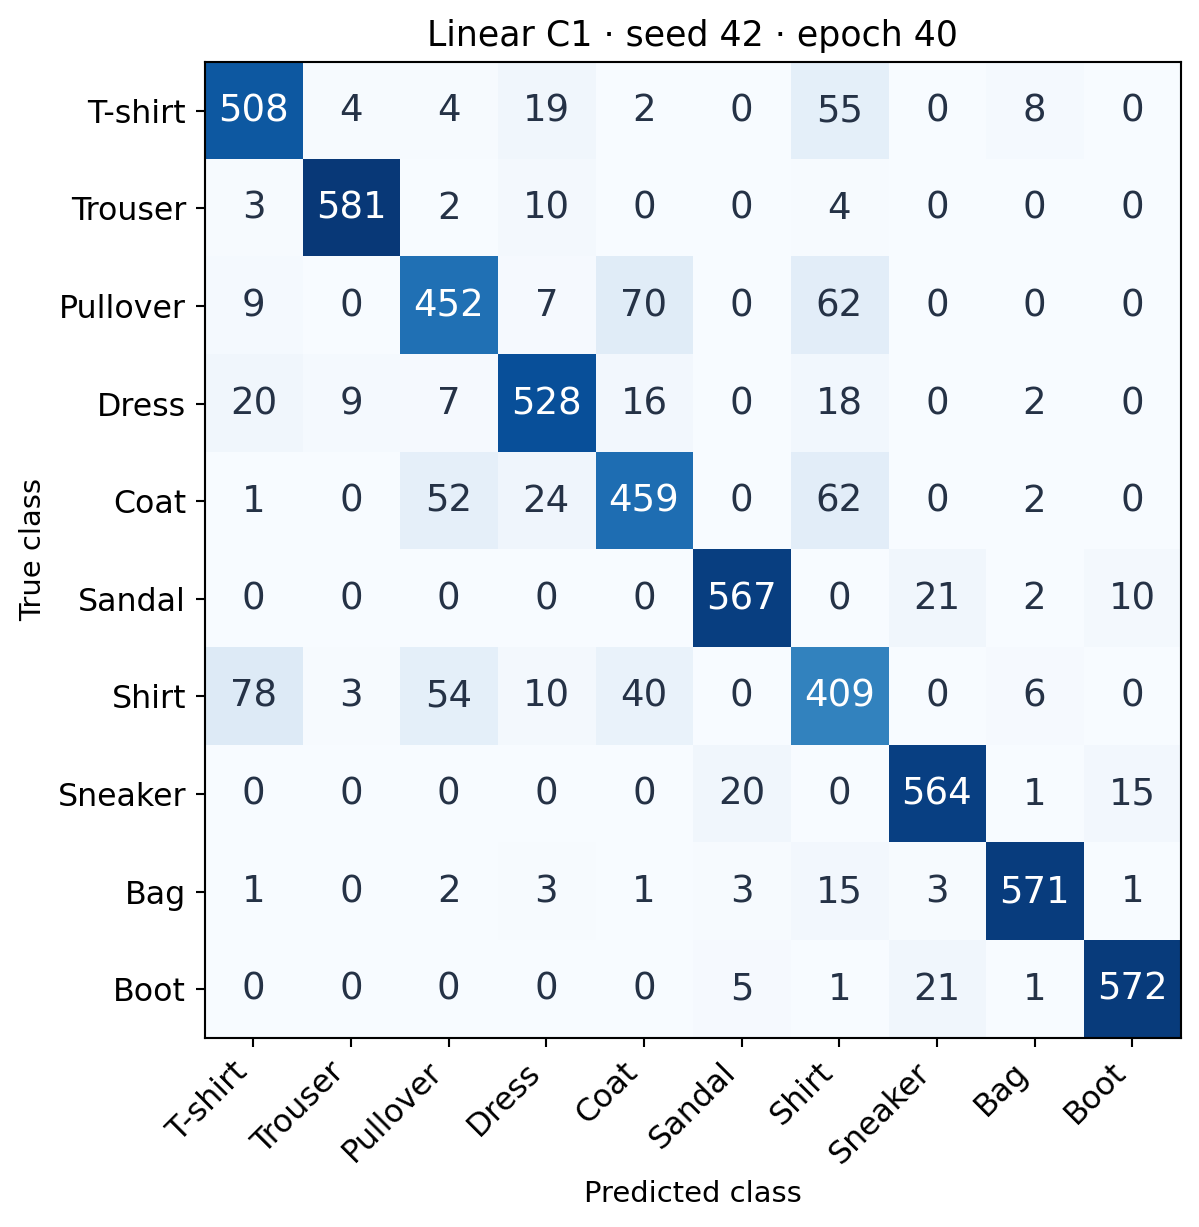
\includegraphics[width=0.60\linewidth]{appendix_figures/linear_seed42_confusion.png}
\caption{Linear integer confusion counts on old validation.}
\end{figure}
\begin{figure}[H]\centering
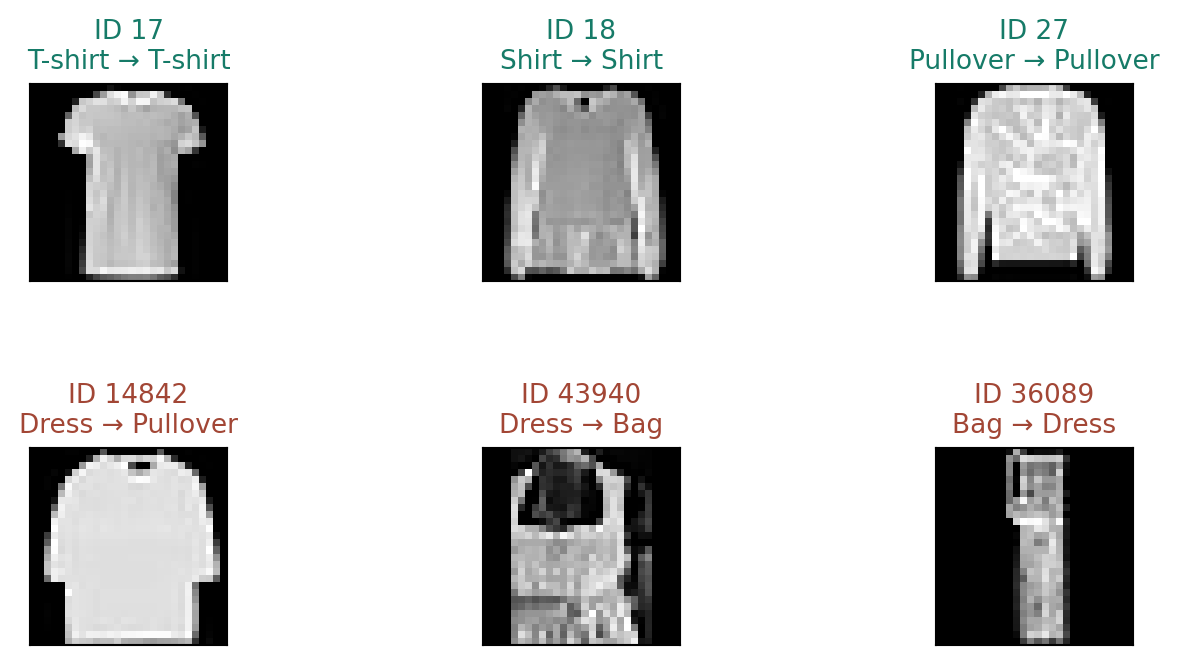
\includegraphics[width=0.68\linewidth]{appendix_figures/linear_seed42_examples.png}
\caption{Linear examples: first three correct IDs (top), three highest-NLL errors (bottom). Titles give true and predicted labels.}
\end{figure}
\clearpage
\subsection{MLP: validation errors and examples}
Recipe C7, seed 42, selected epoch 56: accuracy 91.500\%, macro-F1 91.501\%. Each true class contributes 600 images. The largest off-diagonal counts are 
Shirt $\rightarrow$ T-shirt: 56/600 (9.33\%); T-shirt $\rightarrow$ Shirt: 48/600 (8.00\%); Pullover $\rightarrow$ Coat: 45/600 (7.50\%).
\begin{figure}[H]\centering
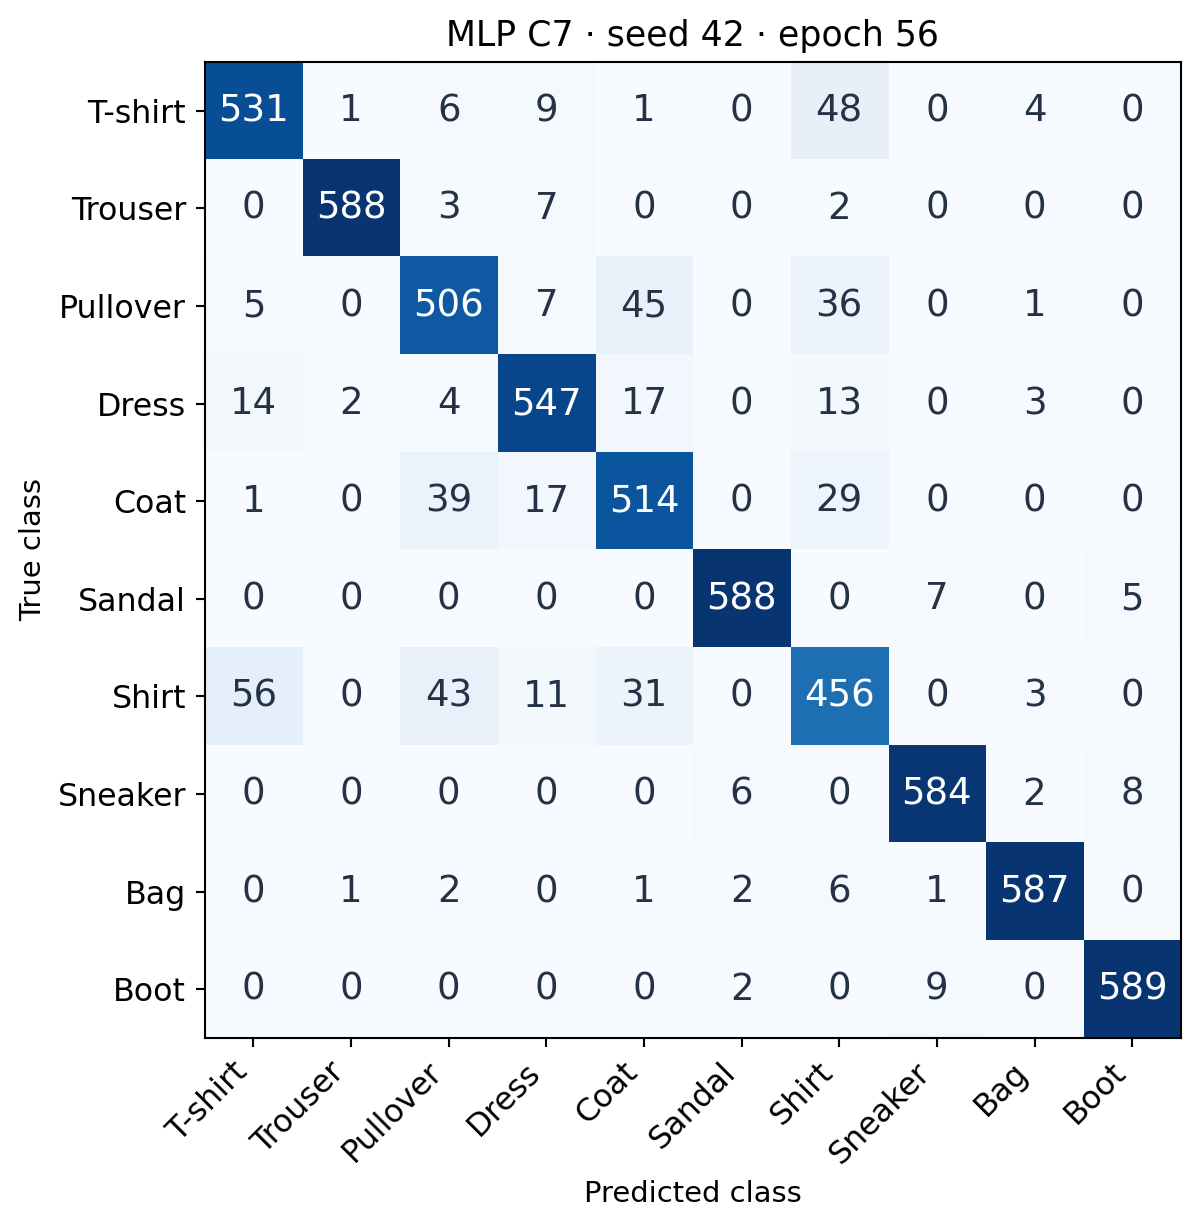
\includegraphics[width=0.60\linewidth]{appendix_figures/mlp_seed42_confusion.png}
\caption{MLP integer confusion counts on old validation.}
\end{figure}
\begin{figure}[H]\centering
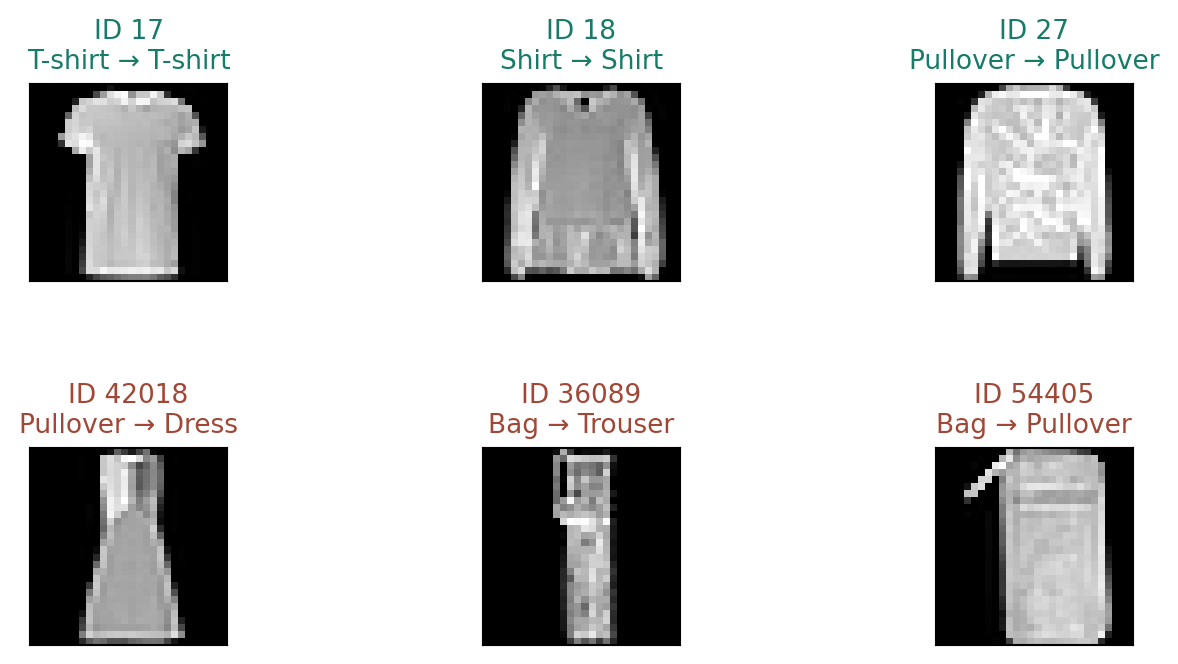
\includegraphics[width=0.68\linewidth]{appendix_figures/mlp_seed42_examples.png}
\caption{MLP examples: first three correct IDs (top), three highest-NLL errors (bottom). Titles give true and predicted labels.}
\end{figure}
\clearpage
\subsection{GRU: validation errors and examples}
Recipe C1, seed 42, selected epoch 37: accuracy 91.350\%, macro-F1 91.324\%. Each true class contributes 600 images. The largest off-diagonal counts are 
Shirt $\rightarrow$ T-shirt: 59/600 (9.83\%); T-shirt $\rightarrow$ Shirt: 52/600 (8.67\%); Pullover $\rightarrow$ Coat: 46/600 (7.67\%).
\begin{figure}[H]\centering
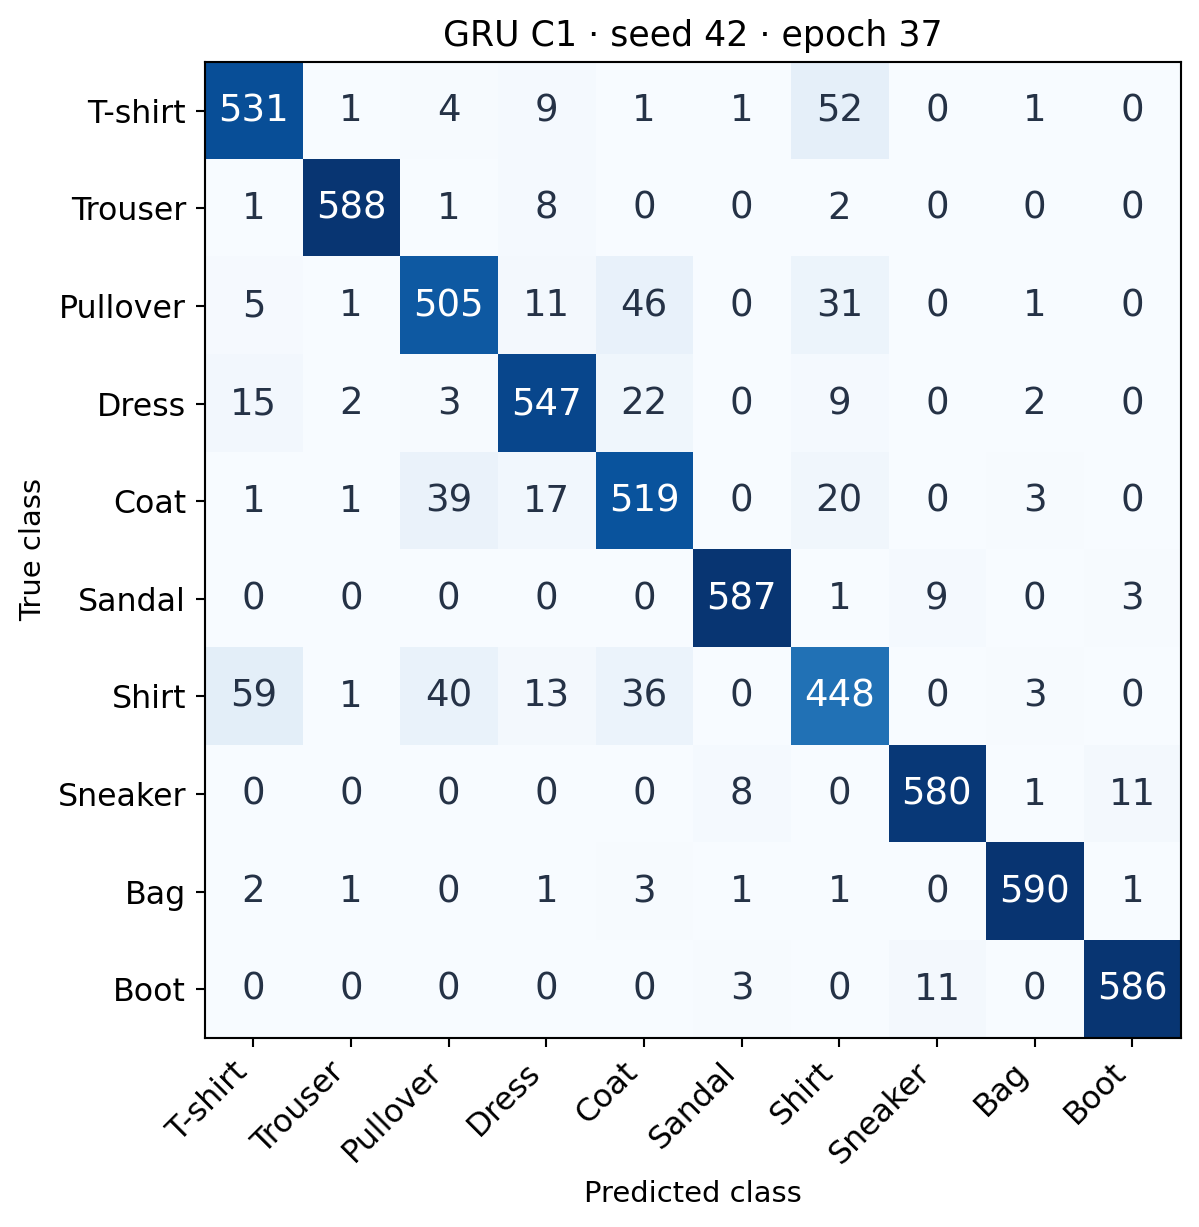
\includegraphics[width=0.60\linewidth]{appendix_figures/gru_seed42_confusion.png}
\caption{GRU integer confusion counts on old validation.}
\end{figure}
\begin{figure}[H]\centering
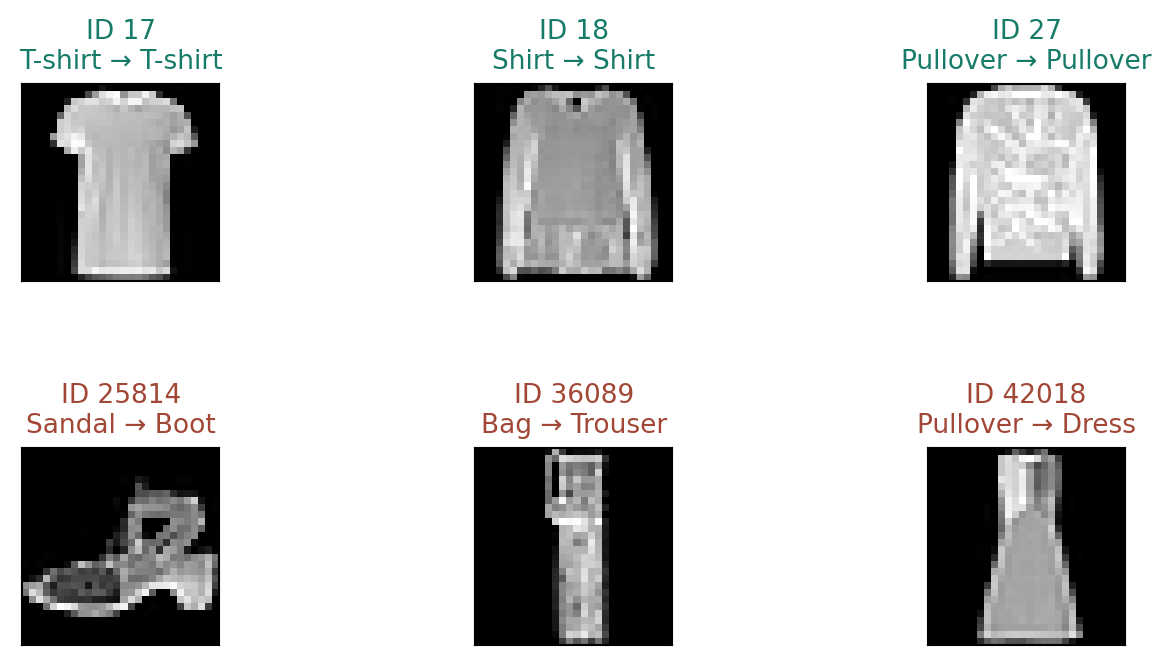
\includegraphics[width=0.68\linewidth]{appendix_figures/gru_seed42_examples.png}
\caption{GRU examples: first three correct IDs (top), three highest-NLL errors (bottom). Titles give true and predicted labels.}
\end{figure}
\clearpage
\subsection{Transformer: validation errors and examples}
Recipe C1, seed 42, selected epoch 58: accuracy 91.567\%, macro-F1 91.541\%. Each true class contributes 600 images. The largest off-diagonal counts are 
Shirt $\rightarrow$ T-shirt: 54/600 (9.00\%); T-shirt $\rightarrow$ Shirt: 41/600 (6.83\%); Coat $\rightarrow$ Pullover: 39/600 (6.50\%).
\begin{figure}[H]\centering
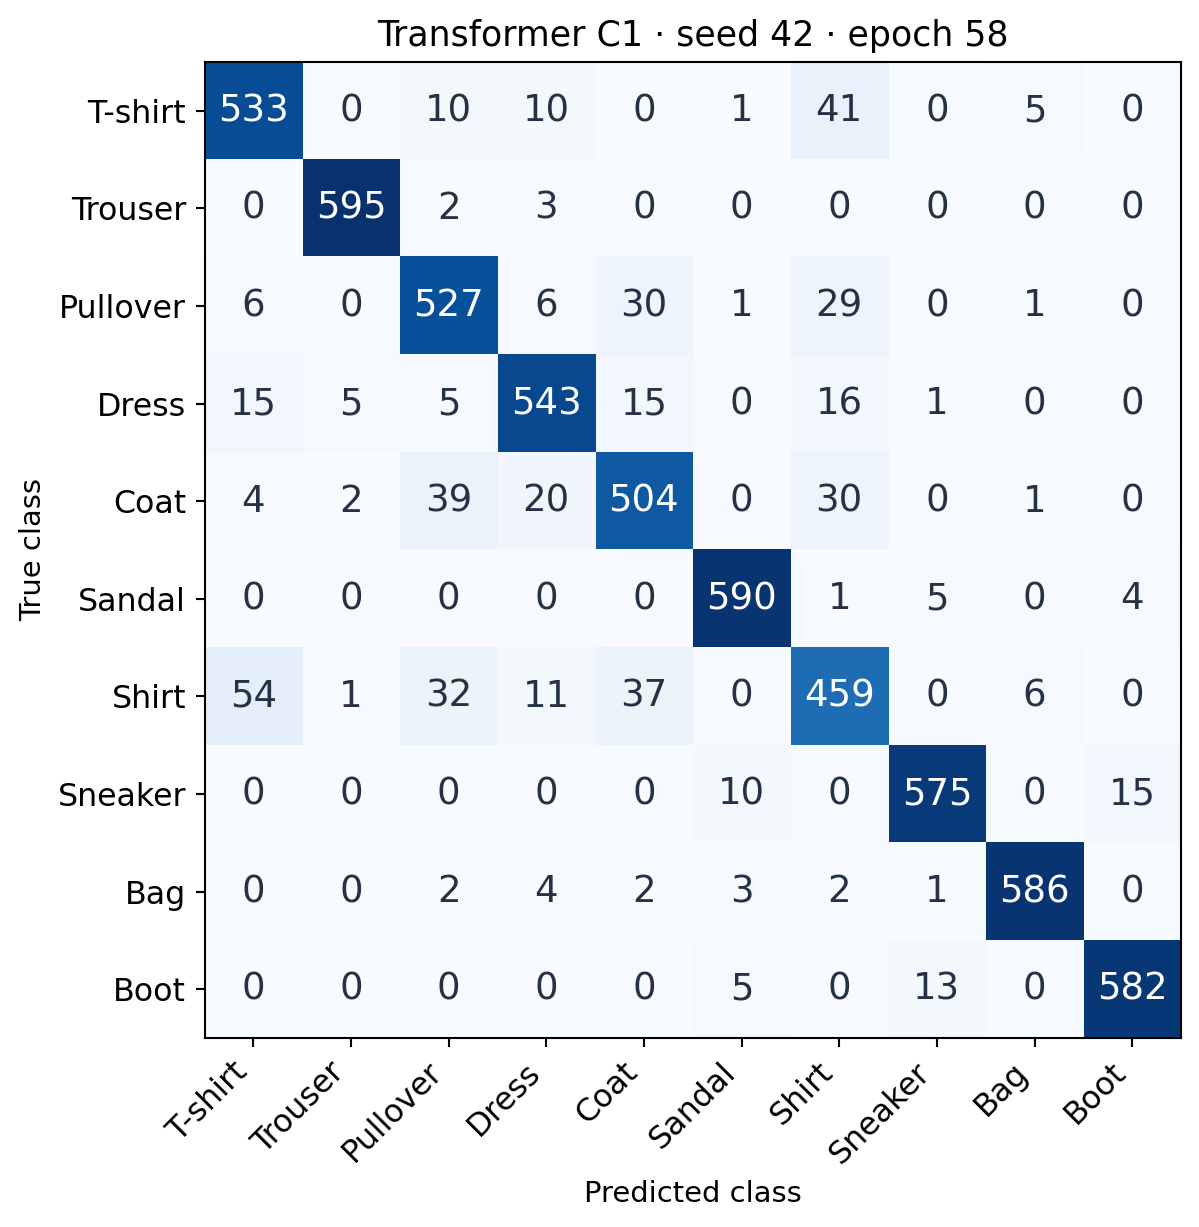
\includegraphics[width=0.60\linewidth]{appendix_figures/transformer_seed42_confusion.png}
\caption{Transformer integer confusion counts on old validation.}
\end{figure}
\begin{figure}[H]\centering
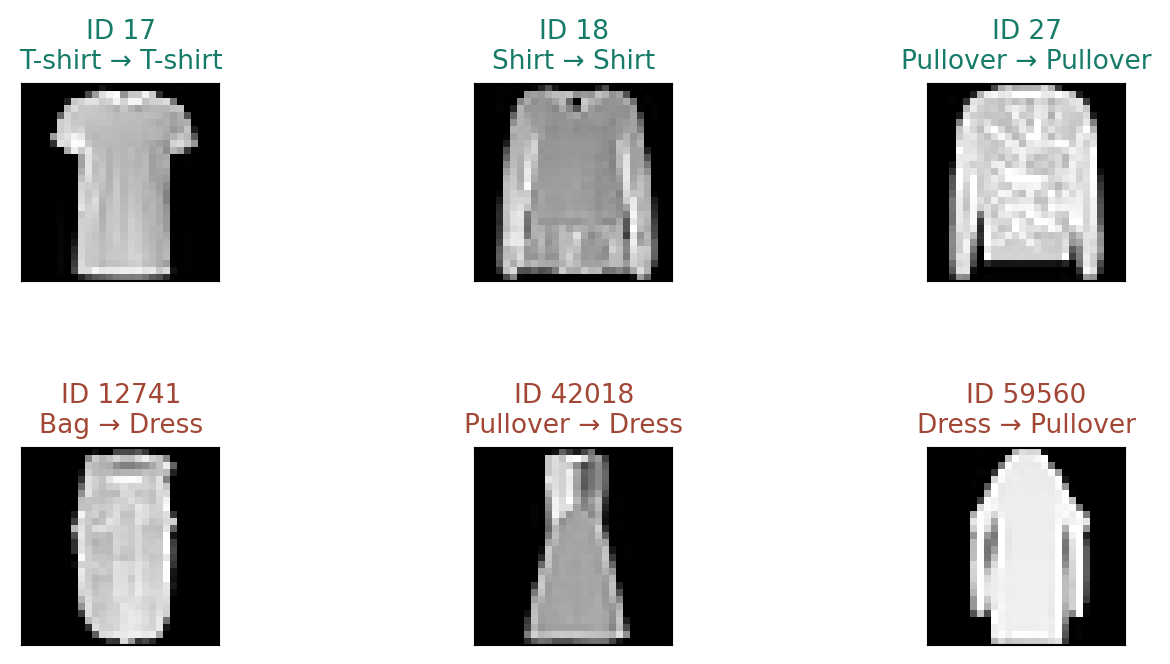
\includegraphics[width=0.68\linewidth]{appendix_figures/transformer_seed42_examples.png}
\caption{Transformer examples: first three correct IDs (top), three highest-NLL errors (bottom). Titles give true and predicted labels.}
\end{figure}
\endgroup

\clearpage
\begin{thebibliography}{99}
\bibitem{fashionmnist}
H. Xiao, K. Rasul and R. Vollgraf.
\emph{Fashion-MNIST: a Novel Image Dataset for Benchmarking Machine Learning Algorithms}. 2017.
\url{https://arxiv.org/abs/1708.07747}.

\bibitem{gru}
K. Cho et al.
\emph{Learning Phrase Representations using RNN Encoder--Decoder for Statistical Machine Translation}. 2014.
\url{https://arxiv.org/abs/1406.1078}.

\bibitem{attention}
A. Vaswani et al.
\emph{Attention Is All You Need}. 2017.
\url{https://arxiv.org/abs/1706.03762}.

\bibitem{adam}
D. P. Kingma and J. Ba.
\emph{Adam: A Method for Stochastic Optimization}. 2014.
\url{https://arxiv.org/abs/1412.6980}.

\bibitem{adamw}
I. Loshchilov and F. Hutter.
\emph{Decoupled Weight Decay Regularization}. 2017.
\url{https://arxiv.org/abs/1711.05101}.

\bibitem{optuna}
T. Akiba et al.
\emph{Optuna: A Next-generation Hyperparameter Optimization Framework}. 2019.
\url{https://arxiv.org/abs/1907.10902}.

\bibitem{fashionpedia}
M. Jia et al.
\emph{Fashionpedia: Ontology, Segmentation, and an Attribute Localization Dataset}. ECCV, 2020.
\url{https://www.ecva.net/papers/eccv_2020/papers_ECCV/papers/123460307.pdf}.

\bibitem{mobilenetv3}
A. Howard et al.
\emph{Searching for MobileNetV3}. ICCV, 2019.
\url{https://openaccess.thecvf.com/content_ICCV_2019/html/Howard_Searching_for_MobileNetV3_ICCV_2019_paper.html}.

\bibitem{temperature}
C. Guo, G. Pleiss, Y. Sun and K. Q. Weinberger.
\emph{On Calibration of Modern Neural Networks}. ICML, PMLR 70, 2017.
\url{https://proceedings.mlr.press/v70/guo17a.html}.

\bibitem{exactbinomial}
C. J. Clopper and E. S. Pearson. The Use of Confidence or Fiducial Limits Illustrated in the Case of the Binomial. Biometrika, 26(4), 1934. Exact-binomial implementation reference: \url{https://docs.scipy.org/doc/scipy-1.16.1/reference/generated/scipy.stats._result_classes.BinomTestResult.proportion_ci.html}.
\end{thebibliography}

